\documentclass{bredelebeamer}
\usepackage{graphicx}
\usepackage{amsmath,amsfonts,amsthm}
\usepackage{hyperref}
\usepackage{setspace}
\usepackage{makecell}
%\usepackage{media9} % for movies
%\usepackage{multimedia} % for movies
\usepackage{caption} % for figure caption
\usepackage{animate}
\usepackage[final]{listings} % for listing source code
\usefonttheme[onlymath]{serif} % make the equations look better
% define box for listing
\definecolor{myblue}{HTML}{4C72B0}
\definecolor{myred}{HTML}{C54E52}
\definecolor{mygreen}{HTML}{56A968}
\lstset{
      language=C++,
      basicstyle=\ttfamily,
      frame=single,
      columns=flexible,
      breaklines=true,
      commentstyle=\color{mygreen},
      keywordstyle = \color{myblue},
      stringstyle  = \color{orange},
      }
\usepackage[absolute,overlay]{textpos} 
\setlength{\parskip}{0.9em}
\setbeamertemplate{navigation symbols}{}
\newcommand*\dif{\mathop{}\!\mathrm{d}}
%%%%%%%%% some settings
\captionsetup[figure]{labelformat=empty} % remove the prefix 'figure' for figure caption
\captionsetup[table]{labelformat=empty} % remove the prefix 'table' for figure caption
\setbeamertemplate{headline}{} %%%%%%%%%%% remove header %%%%%%%%%%%
\setbeamerfont{frametitle}{size=\Large} %% title font size

%%%%%%%%%% title
\title[ ]{DAFoam Workshop 2022}
\subtitle{v3.0.0}

\author{Ping He and Bernardo Pacini \\ ~ \\June 8, 2022 }


\date[June 8, 2022]{}

\setbeamercolor{title}{fg=Black,bg=White!0}
\setbeamercolor{frametitle}{fg=Black,bg=White!0}
%gets rid of footer
%will override 'frame number' instruction above
%comment out to revert to previous/default definitions
\setbeamertemplate{footline}[page number]

\begin{document}

%---------------------------------------------------------------%
\begin{frame}
  \titlepage
\end{frame}

%---------------------------------------------------------------%


%---------------------------------------------------------------%
\begin{frame}{Objectives}

After this workshop, you should be able to
\begin{itemize}
  \setlength\itemsep{1em}
 \item Get familiar with the new features and interfaces in DAFoam v3
 \item Run aerodynamic \& aerostructural optimizations with DAFoam v3
 \item Modify/add DAFoam's C++ and Python codes for a new feature
\end{itemize}

\end{frame}
%---------------------------------------------------------------%

%---------------------------------------------------------------%
\begin{frame}{A few notes}

  \begin{itemize}
    \setlength\itemsep{1em}
   \item We assume you are familiar with DAFoam v2.
   \item This workshop has \textbf{hands-on} examples.
   \item \textbf{Stop} us at any time if you have questions.
   \item The online meeting will be \textbf{recorded}.
   \item All the materials are available at \url{https://github.com/dafoam/workshops}.
\end{itemize}
  
\end{frame}
%---------------------------------------------------------------%

%---------------------------------------------------------------%
\begin{frame}{Outline}
  \tableofcontents
\end{frame}
%---------------------------------------------------------------%

% ************************************************************************************
\section{DAFoam v3 Introduction}
\renewcommand{\arraystretch}{2}

%---------------------------------------------------------------%
\begin{frame}{}
  \center \Large DAFoam v3 Introduction
\end{frame}
%---------------------------------------------------------------%

%---------------------------------------------------------------%
\begin{frame}{What is DAFoam?}

  {\large DAFoam: \textbf{D}iscrete \textbf{A}djoint with Open\textbf{FOAM}}

  ~

  DAFoam develops an efficient discrete adjoint method to perform high-fidelity multidisciplinary design optimization. DAFoam has the following features:
  \center \normalsize
  \begin{itemize}
    \setlength\itemsep{1em}
    \item It uses a popular open-source package OpenFOAM (\url{www.openfoam.com}) for multiphysics analysis
    \item It implements a Jacobian-free discrete adjoint approach with competitive speed, scalability, and accuracy
    \item It has a convenient Python interface to couple with OpenMDAO (\url{www.openmdao.org}) for multidisciplinary design optimization
  \end{itemize}

\end{frame}
%---------------------------------------------------------------%

%---------------------------------------------------------------%
\begin{frame}{What is new in DAFoam v3?}
  DAFoam v3 is a major release that integrated DAFoam and OpenMDAO for multidisciplinary design optimization (MDO) through the OpenMDAO/Mphys interface

  \begin{itemize}
    \setlength\itemsep{1em}
    \item It developed a new Python interface (mphys/mphys\_dafoam.py) to Mphys and OpenMDAO for MDO
    \item Most of the settings are same as v2, but DAFoam v3 uses very different runScript.py because it is coupled with OpenMDAO.
    \item You need to update dependency versions for MDO in v3. Check the DAFoam website (\url{https://dafoam.github.io}).
    \item DAFoam v3 is compatible with all v2 run scripts.
  \end{itemize}
  
\end{frame}
%---------------------------------------------------------------%


% ************************************************************************************
\section{An OpenMDAO tutorial}
\renewcommand{\arraystretch}{2}

%---------------------------------------------------------------%
\begin{frame}{}
  \center \Large An OpenMDAO tutorial

  \normalsize
  Before using DAFoam v3, we need to learn how OpenMDAO works.
  Refer to OpenMDAO's documentation for more advanced usage. \\ 
  \url{https://openmdao.org/newdocs/versions/latest/main.html}
\end{frame}
%---------------------------------------------------------------%

%---------------------------------------------------------------%
\begin{frame}[fragile]{Optimizing a two-component system}
  \begin{figure}
    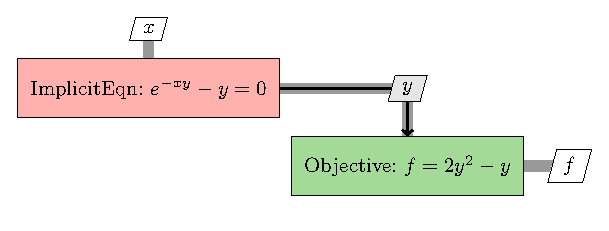
\includegraphics[width=\linewidth]{images/example_xdsm.pdf} 
    \caption{Design structure diagram for the two-component system. The red component is implicit and the green one is explicit. The design variable is $x$ and the objective function is $f$. $y$ is the solution from the implicit component and is passed to the explicit component as the input to compute $f$.}
  \end{figure}
\end{frame}
%---------------------------------------------------------------%


%---------------------------------------------------------------%
\begin{frame}[fragile]{Download DAFoam Docker image and examples}

  The most general way to run the above case is to use the DAFoam Docker image, which has OpenMDAO installed already.

  First, install Docker following this website: \\ \vspace{0.1in} \small \url{https://dafoam.github.io/mydoc_get_started_download_docker.html} \normalsize

  Once done, verify the installation by running:
  \footnotesize
  \lstset{ language=bash }
  \begin{lstlisting}
docker --version
  \end{lstlisting}
  \normalsize
     
  Then run this command to download the DAFoam Docker image: 

  \footnotesize
  \lstset{ language=bash }
  \begin{lstlisting}
docker pull dafoam/opt-packages:v3.0.0
  \end{lstlisting}
  \normalsize
  
  Finally, download the workshop examples at: \\ \vspace{0.1in}
  \small \texttt{\url{https://github.com/dafoam/workshops}}

\end{frame}
%---------------------------------------------------------------%


%---------------------------------------------------------------%
\begin{frame}[fragile]{Start a Docker container}

  If you use Linux or MacOS, open a terminal and use the \texttt{cd} command to go this folder on your local computer. If you put the workshops folder in the \$HOME directory, the command may look like:

  \footnotesize
  \begin{lstlisting}
cd $HOME/workshops/2022_Summer/examples/openmdao
  \end{lstlisting}
  \normalsize
  
  Then, run this command to start a Docker container:

  \footnotesize
  \begin{lstlisting}
docker run -it --rm -u dafoamuser --mount \
"type=bind,src=$(pwd),target=/home/dafoamuser/mount" \ 
-w /home/dafoamuser/mount dafoam/opt-packages:v3.0.0 bash
  \end{lstlisting}
  \normalsize

  If you use Windows, open the Prompt Command terminal, use the \texttt{cd} command to go to the above folder, and run this command: \\ \vspace{0.1in}

  \footnotesize
  \begin{lstlisting}
docker run -it --rm -u dafoamuser --mount \
"type=bind,src=%cd%,target=/home/dafoamuser/mount" \
-w /home/dafoamuser/mount dafoam/opt-packages:v3.0.0 bash
  \end{lstlisting}
  \normalsize

  Once in a Docker container, you should see something like:
  \footnotesize
  \lstset{ language=bash }
  \begin{lstlisting}
dafoamuser@cddb89839078:~/mount$ 
  \end{lstlisting}
  \normalsize

\end{frame}
%---------------------------------------------------------------%



%---------------------------------------------------------------%
\begin{frame}[fragile]{Run the case}

  Once in the docker container, use the \texttt{ls} command to check if you are in the correct directory. You should see something like this:

  \footnotesize
  \begin{lstlisting}
dafoamuser@cddb89839078:~/mount$ ls
runScript.py
  \end{lstlisting}
  \normalsize

  Finally, you can run the case with this command:

  \footnotesize
  \begin{lstlisting}
python runScript.py
  \end{lstlisting}
  \normalsize

  Expected output:

  \footnotesize
  \begin{lstlisting}
dafoamuser@cddb89839078:~/mount$ python runScript.py 
Optimization terminated successfully    (Exit mode 0)
            Current function value: [0.87500003]
            Iterations: 11
            Function evaluations: 11
            Gradient evaluations: 11
Optimization Complete
-----------------------------------
f_opt: [0.87500003]
x_opt: [5.54015542]
  \end{lstlisting}
  \normalsize

\end{frame}
%---------------------------------------------------------------%


%---------------------------------------------------------------%
\begin{frame}[fragile]{An alternative option without Docker}

If you already have a Python 3 on your computer, you can directly run the OpenMDAO case without using the Docker. First, load your Python 3 environment, and run this command in your terminal to install OpenMDAO
  \footnotesize
  \lstset{ language=bash }
  \begin{lstlisting}
pip install openmdao==3.16.0
  \end{lstlisting}
  \normalsize
     
  Then go to the tutorial folder:

  \footnotesize
  \begin{lstlisting}
cd $HOME/workshops/2022_Summer/examples/openmdao
  \end{lstlisting}
  \normalsize

  And run the case:

  \footnotesize
  \lstset{ language=bash }
  \begin{lstlisting}
python runScript.py
  \end{lstlisting}
  \normalsize

\end{frame}
%---------------------------------------------------------------%

%---------------------------------------------------------------%
\begin{frame}[fragile]{N2 diagram}
  After the case is finished, you should see a N2 diagram (n2.html) generated for this case. The runScript.py file essential sets the components and their data transfer (connection) for the optimization.
  \begin{figure}
    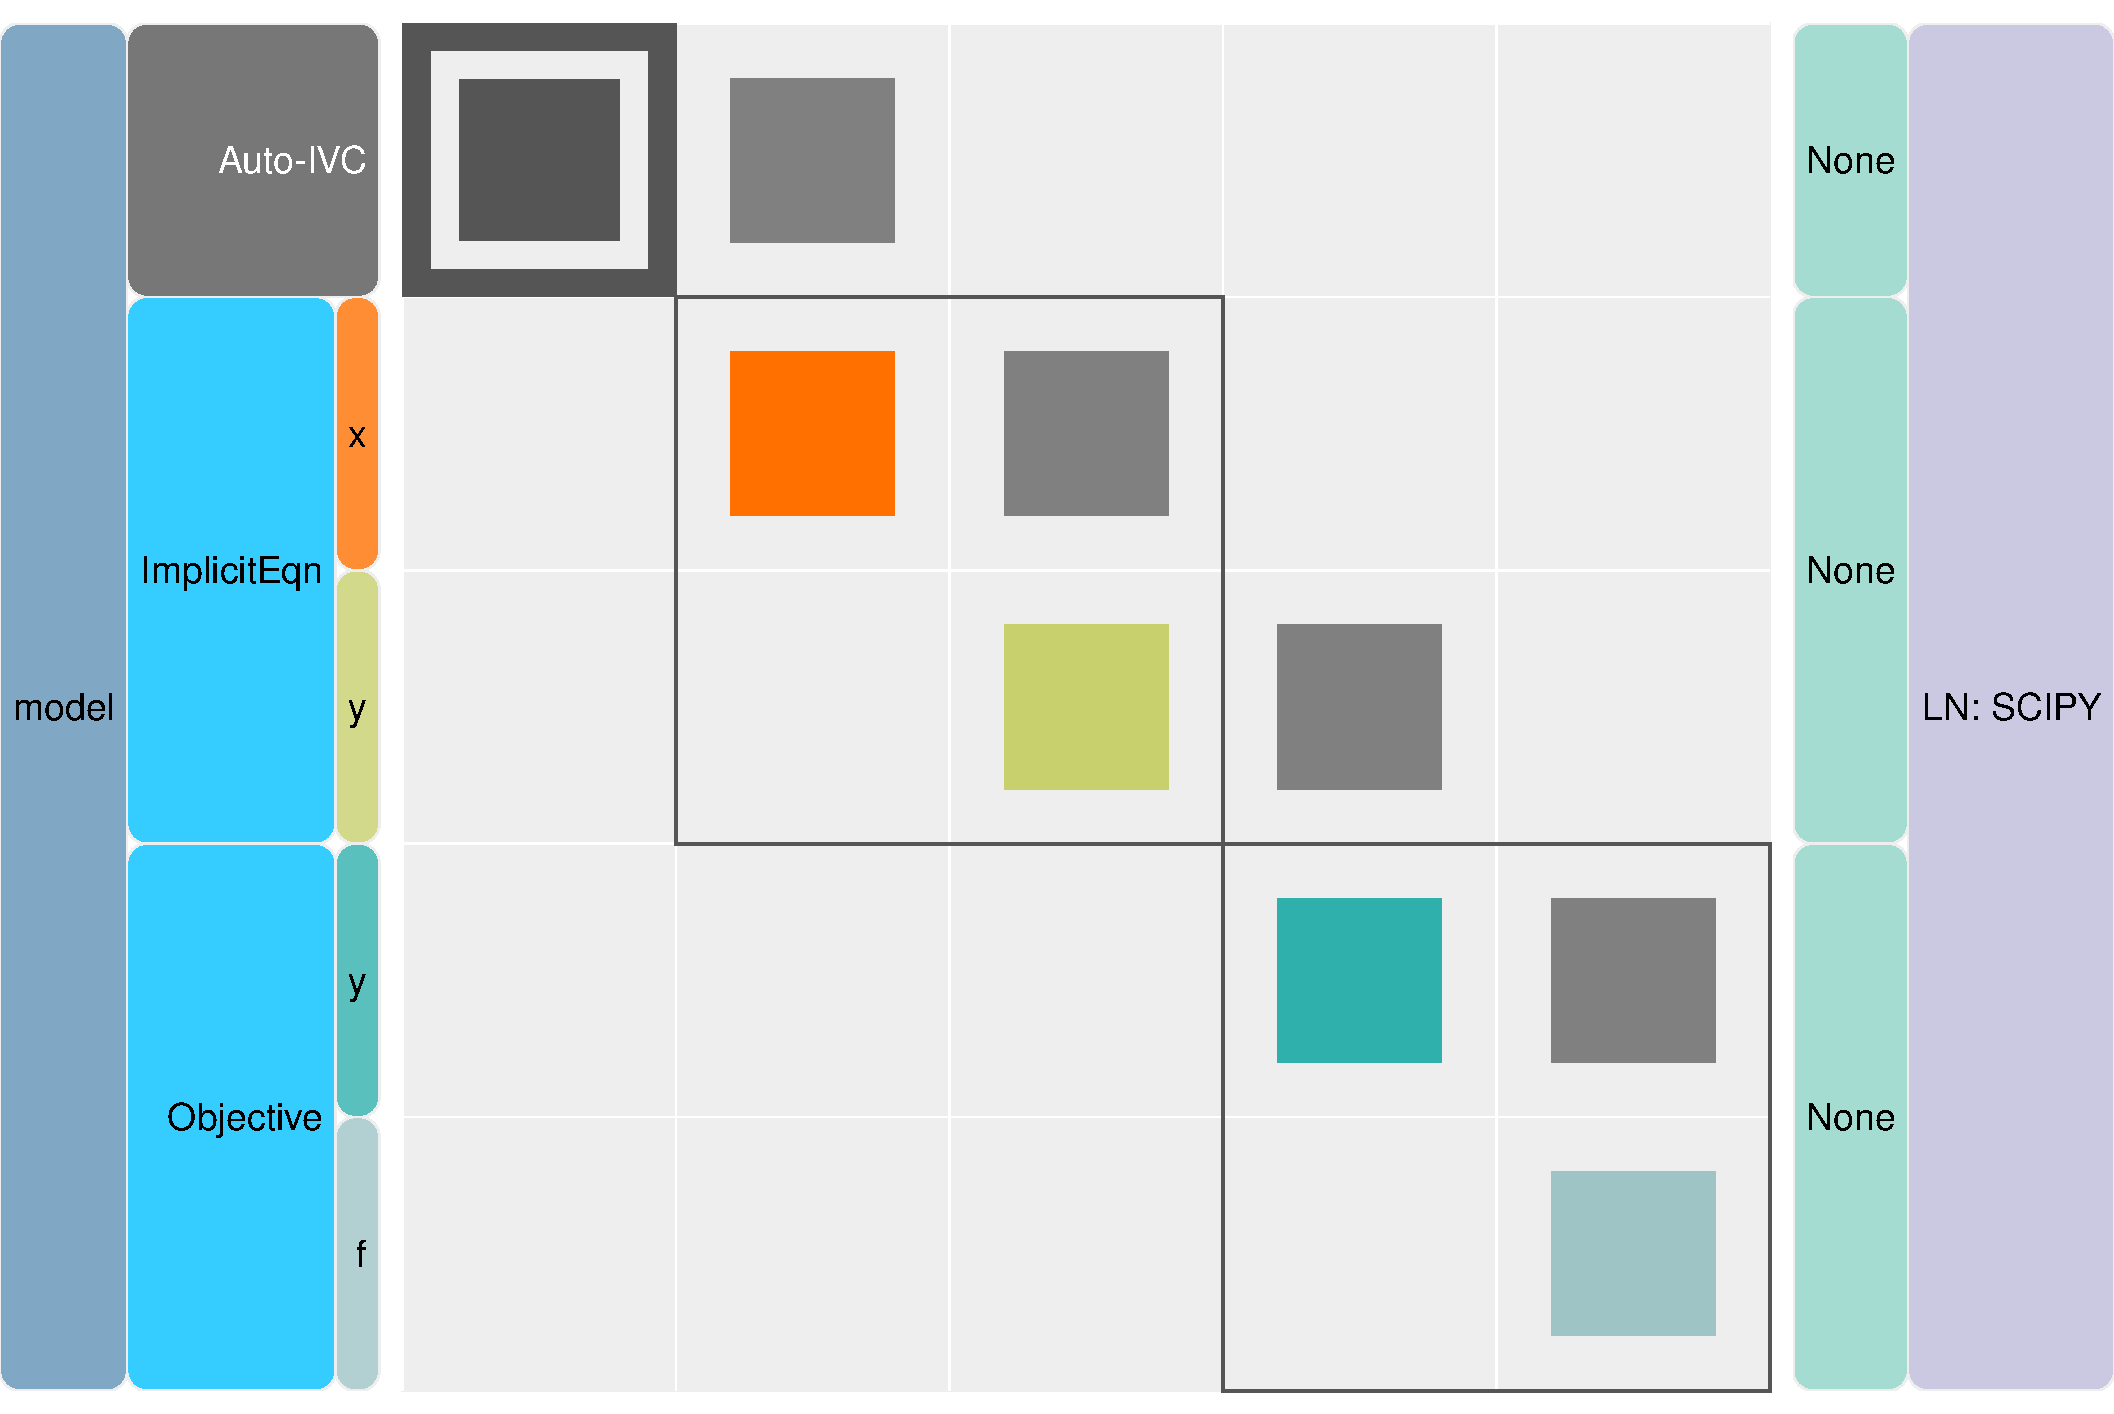
\includegraphics[width=0.8\linewidth]{images/example_n2.pdf} 
    \caption{The N2 diagram for the two-component optimization.}
  \end{figure}
\end{frame}
%---------------------------------------------------------------%


%---------------------------------------------------------------%
\begin{frame}[fragile]{runScript.py details (1/3)}
  \footnotesize
  \lstset{ language=python }
  \begin{lstlisting}
class ImplicitEqn(om.ImplicitComponent):
    def setup(self):
        # define input
        self.add_input("x", val=1.0)
        # define output
        self.add_output("y", val=1.0)

    def setup_partials(self):
        # Finite difference all partials.
        self.declare_partials("*", "*", method="fd")

    def apply_nonlinear(self, inputs, outputs, residuals):
        # get the input and output and compute the residual
        # R = e^(-x * y) - y
        # NOTE: we use [0] here because OpenMDAO assumes all inputs
        # and outputs are arrays. If the input is a scalar, OpenMDAO
        # will create an array that has size 1, so to get its value
        # we have to use [0]
        x = inputs["x"][0]
        y = outputs["y"][0]
        residuals["y"] = np.exp(-x * y) - y
  \end{lstlisting}
  \normalsize
\end{frame}
%---------------------------------------------------------------%

%---------------------------------------------------------------%
\begin{frame}[fragile]{runScript.py details (2/3)}
  \footnotesize
  \lstset{ language=python }
  \begin{lstlisting}
class Objective(om.ExplicitComponent):
    def setup(self):

        # define input
        self.add_input("y", val=1.0)

        # define output
        self.add_output("f", val=1.0)

    def setup_partials(self):
        # Finite difference all partials.
        self.declare_partials("*", "*", method="fd")

    def compute(self, inputs, outputs):
        # compute the output based on the input
        y = inputs["y"][0]

        outputs["f"] = 2 * y * y - y + 1
  \end{lstlisting}
  \normalsize
\end{frame}
%---------------------------------------------------------------%


%---------------------------------------------------------------%
\begin{frame}[fragile]{runScript.py details (3/3)}
  \footnotesize
  \lstset{ language=python }
  \begin{lstlisting}
# create an OpenMDAO problem object
prob = om.Problem()
# now add the implicit component defined above to prob
prob.model.add_subsystem("ImplicitEqn", ImplicitEqn(), promotes=["*"])
# add the objective explicit component defined above to prob
prob.model.add_subsystem("Objective", Objective(), promotes=["*"],)
# set the linear/nonlinear equation solution for the implicit component
prob.model.nonlinear_solver = om.NewtonSolver(solve_subsystems=False)
prob.model.linear_solver = om.ScipyKrylov()
# set the design variable and objective function
prob.model.add_design_var("x", lower=-10, upper=10)
prob.model.add_objective("f", scaler=1)
# setup the optimizer
prob.driver = om.ScipyOptimizeDriver()
prob.driver.options["optimizer"] = "SLSQP"
# setup the problem
prob.setup()
# write the n2 diagram
om.n2(prob, show_browser=False, outfile="n2.html")
# run the optimization
prob.run_driver()
  \end{lstlisting}
  \normalsize
\end{frame}
%---------------------------------------------------------------%

%---------------------------------------------------------------%
\begin{frame}[fragile]{Summary}
  \begin{itemize}
    \setlength\itemsep{1em}
   \item To use OpenMDAO for optimizations, one needs to write classes for each component in the system, define their inputs and outputs, and implement the way to compute the outputs (explicit components) or residuals (implicit components). 
   \item Then one needs to add these components to the optimization problem in the run script, set their connection, set the design variables, objective and constraint functions, and run the optimization.
   \item A new open-source interface Mphys was recently developed (\url{https://github.com/openmdao/mphys}) to rewrite the MACH-Aero modules' interfaces (e.g., pyGeo, IDWarp) into the OpenMDAO component format. 
   \item DAFoam v3 has a Python interface to OpenMDAO/Mphys (dafoam/mphys/mphys\_dafoam.py). So to run optimizations with DAFoam v3, one needs to use the new run script that sets the components, data transfer, design variables, objective and constraint functions in the optimization (see next section).
  \end{itemize}
\end{frame}
%---------------------------------------------------------------%


% ************************************************************************************
\section{Aerodynamic optimization}
\renewcommand{\arraystretch}{2}

%---------------------------------------------------------------%
\begin{frame}{}
  \center \Large Aerodynamic optimization
\end{frame}
%---------------------------------------------------------------%



%---------------------------------------------------------------%
\begin{frame}{Summary of the NACA0012 subsonic case}

  \begin{table}
    \renewcommand{\arraystretch}{1.5}
    \small
    \centering
    \label{tab:implemented_models}
    \begin{tabular}{llllllllllll}
    \hline
    Optimizer   & IPOPT \\
    Flow and adjoint solvers  & DARhoSimpleFoam  \\
    Geometry  & NACA0012 \\
    Mesh  & 4\,032 cells\\
    Objective function  & $C_d$ \\
    Design variables & 20 FFDs and $\alpha$ \\
    Constraint & $C_l=0.5$, thickness, volume, TE/LE \\
    $U_\infty$  & 100 m/s \\
    $Re$  & 6.7$\times10^6$\\
    Turbulence Model  & Spalart--Allmaras\\
     \hline
    \end{tabular}
  \end{table}

  You can find the case settings in workshops/2022\_Summer/examples/naca0012.
\end{frame}
%---------------------------------------------------------------%


%---------------------------------------------------------------%
\begin{frame}[fragile]{Run the case}

  First, use the \texttt{cd} command to go the workshops/2022\_Summer/examples/naca0012 folder. Then, use the command in Slide 11 to start a Docker container. Next, use the \texttt{ls} command to check if you are in the correct directory.
  \footnotesize
  \lstset{ language=bash }
  \begin{lstlisting}
dafoamuser@bd114f3f7c94:~/mount$ ls
0.orig       FFD       genAirFoilMesh.py  preProcessing.sh  runScript.py
Allclean.sh  constant  paraview.foam      profiles          system
  \end{lstlisting}
  \normalsize

  Next, run this command to generate the mesh:
  \footnotesize
  \lstset{ language=bash }
  \begin{lstlisting}
./preProcessing.sh
  \end{lstlisting}
  \normalsize

  Finally, run the optimization with 2 cores.
  \footnotesize
  \lstset{ language=bash }
  \begin{lstlisting}
mpirun -np 2 python runScript.py 2>&1 | tee logOpt.txt
  \end{lstlisting}
  \normalsize

  The optimization log will be printed to the screen and saved to \texttt{logOpt.txt}. In addition, the optimizer will write a separate log to the disk \texttt{opt\_IPOPT.txt}.

\end{frame}
%---------------------------------------------------------------%

%---------------------------------------------------------------%
\begin{frame}[fragile]{How to post-process the optimization results?}

  This has been covered in the 2021 workshop, refer to Slides 29 to 47 from 
  \url{https://github.com/DAFoam/workshops/blob/main/2021_Summer/slides/2021_Summer_Workshop.pdf}

\end{frame}
%---------------------------------------------------------------%


%---------------------------------------------------------------%
\begin{frame}[fragile]{NACA0012 N2 diagram}

  \begin{figure}
    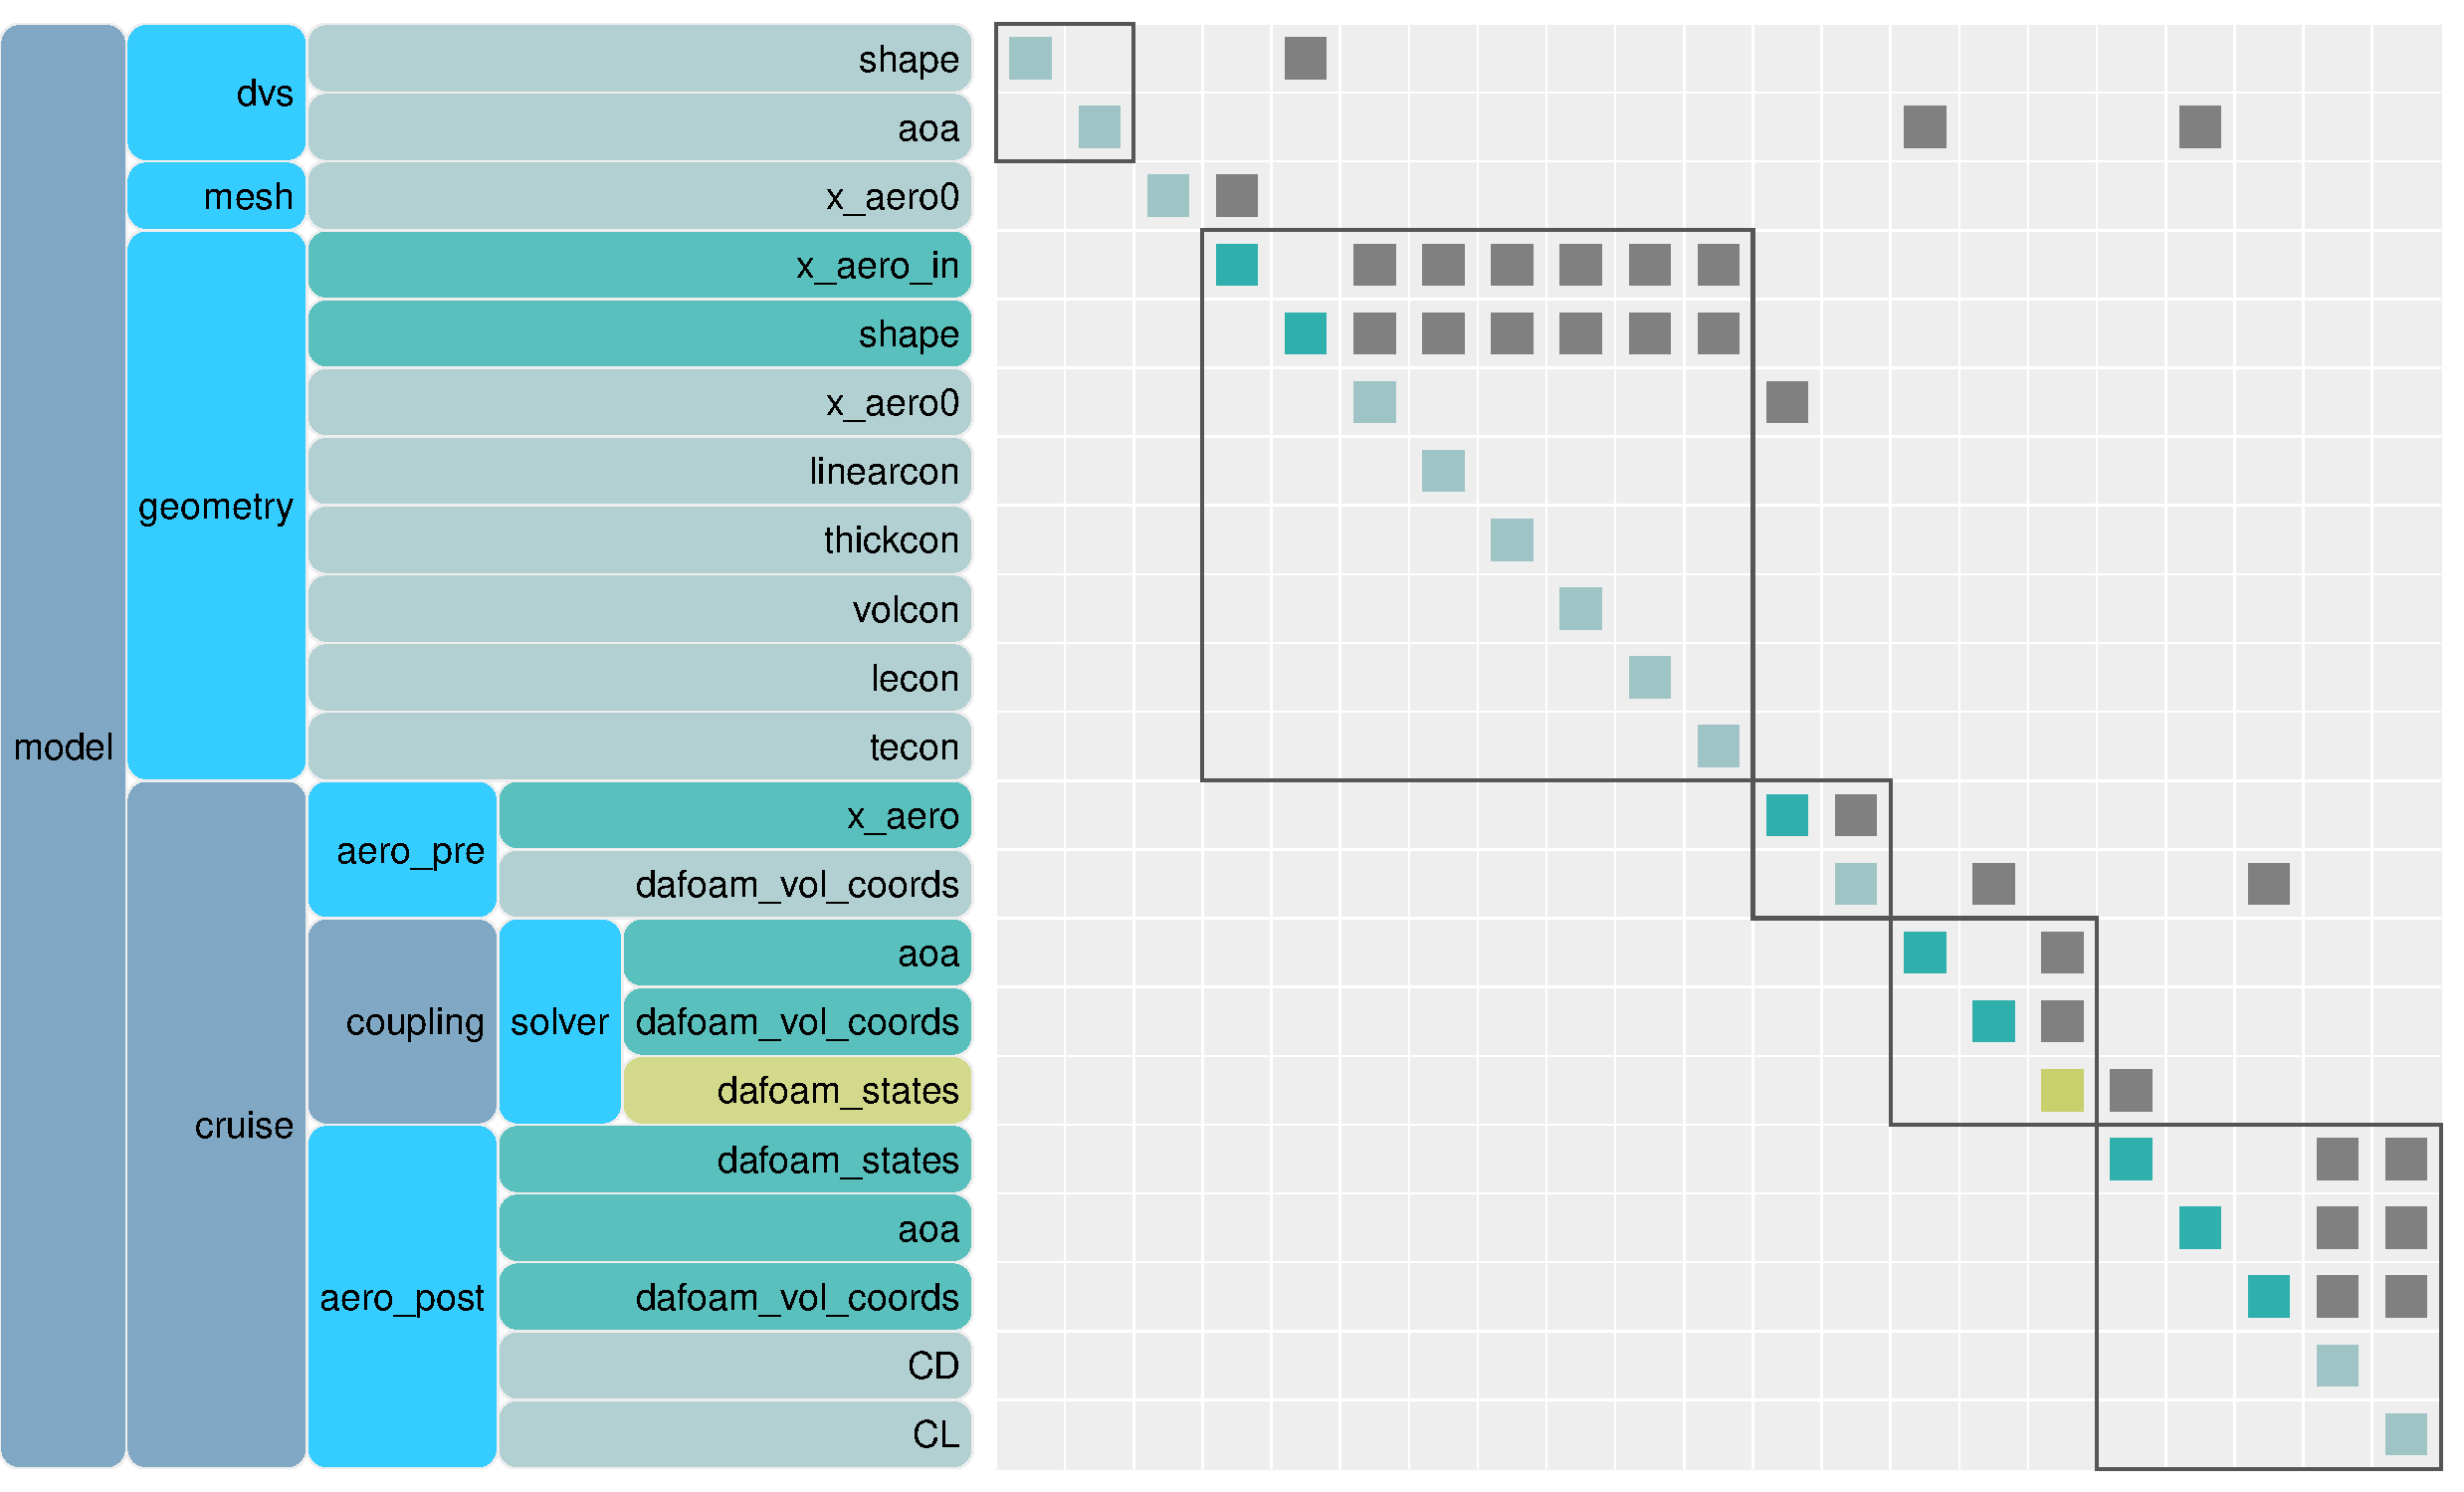
\includegraphics[width=\linewidth]{images/naca0012_n2.pdf} 
    \caption{The N2 diagram for the NACA0012 aerodynamic optimization.}
  \end{figure}

\end{frame}
%---------------------------------------------------------------%


%---------------------------------------------------------------%
\begin{frame}[fragile]{runScript.py details (1/10)}
Most of the settings in DAFoam v3 are same as v2. The main difference is that DAFoam v3 uses a very different runScript.py
  \footnotesize
  \lstset{ language=bash }
  \begin{lstlisting}
# import modules
import os
import argparse
import numpy as np
from mpi4py import MPI
import openmdao.api as om
from mphys.multipoint import Multipoint
from dafoam.mphys import DAFoamBuilder, OptFuncs
from mphys.scenario_aerodynamic import ScenarioAerodynamic
from pygeo.mphys  import OM_DVGEOCOMP
from pygeo import geo_utils
    
# input arguments for runScript.py    
parser = argparse.ArgumentParser()
# which optimizer to use. Options are: IPOPT (default), SLSQP, and SNOPT
parser.add_argument("-optimizer", help="optimizer to use", type=str, default="IPOPT")
# which task to run. Options are: opt (default), runPrimal, runAdjoint, checkTotals
parser.add_argument("-task", help="type of run to do", type=str, default="opt")
args = parser.parse_args()
  \end{lstlisting}
  \normalsize

\end{frame}
%---------------------------------------------------------------%

%---------------------------------------------------------------%
\begin{frame}[fragile]{runScript.py details (2/10)}
  The input parameters, daOptions, meshOptions are same as DAFoam v2. Next, we need to set a Multipoint Top class. We need to add all the components in the \texttt{setup} function.
  \footnotesize
  \lstset{ language=bash }
  \begin{lstlisting}
# Top class to setup the optimization problem
class Top(Multipoint):
    def setup(self):
        # create the builder to initialize the DASolvers
        dafoam_builder = DAFoamBuilder(daOptions, meshOptions, scenario="aerodynamic")
        dafoam_builder.initialize(self.comm)
        # add the design variable component 
        self.add_subsystem("dvs", om.IndepVarComp(), promotes=["*"])
        # add the mesh component
        self.add_subsystem("mesh", dafoam_builder.get_mesh_coordinate_subsystem())
        # add the geometry component (FFD)
        self.add_subsystem("geometry", OM_DVGEOCOMP(ffd_file="FFD/wingFFD.xyz"))
        # add a scenario and pass the builder to it
        self.mphys_add_scenario("cruise", ScenarioAerodynamic(aero_builder=dafoam_builder))
        # need to do manually connection
        self.connect("mesh.x_aero0", "geometry.x_aero_in")
        self.connect("geometry.x_aero0", "cruise.x_aero")
  \end{lstlisting}
  \normalsize
  \end{frame}
%---------------------------------------------------------------%

%---------------------------------------------------------------%
\begin{frame}[fragile]{runScript.py details (3/10)}
Next, we need to do the proper connection and configurations for the above components in the \texttt{configure} function. We also need to set the design variables, objective and constraint functions. The overall process is similar to v2 but it needs to use a different syntax to set up.
    \footnotesize
    \lstset{ language=bash }
    \begin{lstlisting}
def configure(self):
    # configure and setup perform a similar function, i.e., initialize 
    # the optimization. The configure will be run after setup
    # add the objective function to the cruise scenario
    self.cruise.aero_post.mphys_add_funcs()
    # get the surface coordinates from the mesh component
    points = self.mesh.mphys_get_surface_mesh()
    # add pointset to the geometry component
    self.geometry.nom_add_discipline_coords("aero", points)
    # set the triangular points to the geo component for geo constraints
    tri_points = self.mesh.mphys_get_triangulated_surface()
    self.geometry.nom_setConstraintSurface(tri_points)
  \end{lstlisting}
  \normalsize
  \end{frame}
%---------------------------------------------------------------%

%---------------------------------------------------------------%
\begin{frame}[fragile]{runScript.py details (4/10)}
Next, we define an angle of attack (aoa) function to change the far field velocity, and add it to the "cruise" scenario as the design variable.
  \footnotesize
  \lstset{ language=bash }
  \begin{lstlisting}
# define an angle of attack function to change the U direction at the far field
def aoa(val, DASolver):
    aoa = val[0] * np.pi / 180.0
    U = [float(U0 * np.cos(aoa)), float(U0 * np.sin(aoa)), 0]
    # we need to update the U value only
    DASolver.setOption("primalBC", {"U0": {"value": U}})
    DASolver.updateDAOption()

# pass this aoa function to the cruise group
self.cruise.coupling.solver.add_dv_func("aoa", aoa)
self.cruise.aero_post.add_dv_func("aoa", aoa)
  \end{lstlisting}
  \normalsize
  \end{frame}
%---------------------------------------------------------------%

%---------------------------------------------------------------%
\begin{frame}[fragile]{runScript.py details (5/10)}
We can then add the shape as the design variable by choosing all the FFD points. The setup is similar to v2.
  \footnotesize
  \lstset{ language=bash }
  \begin{lstlisting}
# select the FFD points to move
pts = self.geometry.DVGeo.getLocalIndex(0)
indexList = pts[:, :, :].flatten()
PS = geo_utils.PointSelect("list", indexList)
nShapes = self.geometry.nom_addGeoDVLocal(dvName="shape", pointSelect=PS)
  \end{lstlisting}
  \normalsize
  \end{frame}
%---------------------------------------------------------------%

%---------------------------------------------------------------%
\begin{frame}[fragile]{runScript.py details (6/10)}
Because it is a symmetric case, we need to impose the symmetry constraint for the k=0 and k=1 level FFD points. The setup is very similar to v2.
  \footnotesize
  \lstset{ language=bash }
  \begin{lstlisting}
# setup the symmetry constraint to link the y displacement between k=0 and k=1
nFFDs_x = pts.shape[0]
nFFDs_y = pts.shape[1]
indSetA = []
indSetB = []
for i in range(nFFDs_x):
    for j in range(nFFDs_y):
        indSetA.append(pts[i, j, 0])
        indSetB.append(pts[i, j, 1])
self.geometry.nom_addLinearConstraintsShape("linearcon", indSetA, indSetB, factorA=1.0, factorB=-1.0)
  \end{lstlisting}
  \normalsize
  \end{frame}
%---------------------------------------------------------------%

%---------------------------------------------------------------%
\begin{frame}[fragile]{runScript.py details (7/10)}
Similar to v2, we need to set leList and teList for the volume and thickness constraint. We also use the LETE constraint to fix the leading edge and trailing edge.
  \footnotesize
  \lstset{ language=bash }
  \begin{lstlisting}
# setup the volume and thickness constraints
leList = [[1e-4, 0.0, 1e-4], [1e-4, 0.0, 0.1 - 1e-4]]
teList = [[0.998 - 1e-4, 0.0, 1e-4], [0.998 - 1e-4, 0.0, 0.1 - 1e-4]]
self.geometry.nom_addThicknessConstraints2D("thickcon", leList, teList, nSpan=2, nChord=10)
self.geometry.nom_addVolumeConstraint("volcon", leList, teList, nSpan=2, nChord=10)
# add the LE/TE constraints
self.geometry.nom_add_LETEConstraint("lecon", volID=0, faceID="iLow", topID="k")
self.geometry.nom_add_LETEConstraint("tecon", volID=0, faceID="iHigh", topID="k")
  \end{lstlisting}
  \normalsize
  \end{frame}
%---------------------------------------------------------------%

%---------------------------------------------------------------%
\begin{frame}[fragile]{runScript.py details (8/10)}
Now, we can add the shape and aoa variables as the output for the "dvs" component and use them as the design variables. Note that we need to manually connect dvs' output to the cruise and geometry component. See the N2 diagram.
  \footnotesize
  \lstset{ language=bash }
  \begin{lstlisting}
# add the design variables to the dvs component's output
self.dvs.add_output("shape", val=np.array([0] * nShapes))
self.dvs.add_output("aoa", val=np.array([aoa0]))
# manually connect the dvs output to the geometry and cruise
self.connect("aoa", "cruise.aoa")
self.connect("shape", "geometry.shape")

# define the design variables to the top level
self.add_design_var("shape", lower=-1.0, upper=1.0, scaler=1.0)
self.add_design_var("aoa", lower=0.0, upper=10.0, scaler=1.0)
  \end{lstlisting}
  \normalsize
  \end{frame}
%---------------------------------------------------------------%

%---------------------------------------------------------------%
\begin{frame}[fragile]{runScript.py details (9/10)}
Finally, we add the objective and constraint functions.
  \footnotesize
  \lstset{ language=bash }
  \begin{lstlisting}
# add objective and constraints to the top level
self.add_objective("cruise.aero_post.CD", scaler=1.0)
self.add_constraint("cruise.aero_post.CL", equals=CL_target, scaler=1.0)
self.add_constraint("geometry.thickcon", lower=0.5, upper=3.0, scaler=1.0)
self.add_constraint("geometry.volcon", lower=1.0, scaler=1.0)
self.add_constraint("geometry.tecon", equals=0.0, scaler=1.0, linear=True)
self.add_constraint("geometry.lecon", equals=0.0, scaler=1.0, linear=True)
self.add_constraint("geometry.linearcon", equals=0.0, scaler=1.0, linear=True)
  \end{lstlisting}
  \normalsize
  \end{frame}
%---------------------------------------------------------------%

%---------------------------------------------------------------%
\begin{frame}[fragile]{runScript.py details (10/10)}
Once the Top class is created, we pass it as the OpenMDAO problem's model. Then, we can run the OpenMDAO's \texttt{driver} for optimization.
  \footnotesize
  \lstset{ language=bash }
  \begin{lstlisting}
prob = om.Problem()
prob.model = Top()
prob.setup(mode="rev") # reverse mode AD
om.n2(prob, show_browser=False, outfile="mphys.html")
# initialize the optimization function
optFuncs = OptFuncs(daOptions, prob)
# use pyOptSparse to run optimization
prob.driver = om.pyOptSparseDriver()
prob.driver.options["optimizer"] = args.optimizer
# ........... pyOptSparse optimizer setup .........
# set the output option
prob.driver.options["debug_print"] = ["nl_cons", "objs", "desvars"]
# prob.driver.options["print_opt_prob"] = True
prob.driver.hist_file = "OptView.hst"
# select task to run
if args.task == "opt":
    # solve CL by changing aoa
    optFuncs.findFeasibleDesign(["cruise.aero_post.CL"], ["aoa"], targets=[CL_target])
    # run the optimization
    prob.run_driver()
  \end{lstlisting}
  \normalsize
  \end{frame}
%---------------------------------------------------------------%

%---------------------------------------------------------------%
\begin{frame}[fragile]{Summary}
    \begin{itemize}
      \setlength\itemsep{1em}
      \item The runScript.py is essentially an OpenMDAO run script. So we suggest you first learn how OpenMDAO works by going through the OpenMDAO's documentation (\url{https://openmdao.org/newdocs/versions/latest/main.html}).
     \item We can use the above script to run any airfoil aerodynamic optimization with DAFoam v3. If you want to change the flight conditions, FFD points, airfoil profiles, refer to the DAFoam FAQ. \url{https://dafoam.github.io/mydoc_get_started_faq.html}. Note that these changes are for v2 but they also work for v3.
     \item For 3D wing aerodynamic optimization, refer to the run script \url{https://github.com/DAFoam/tutorials/blob/main/MACH_Tutorial_Wing/runScript_Aero.py}
     \item For multipoint optimization, refer to the run script \url{https://github.com/DAFoam/tutorials/blob/main/NACA0012_Airfoil/multipoint/runScript.py}
    \end{itemize}
  \end{frame}
%---------------------------------------------------------------%
  

% ************************************************************************************
\section{Aerostructural optimization}
\renewcommand{\arraystretch}{2}

%---------------------------------------------------------------%
\begin{frame}{}
  \center \Large Aerostructural optimization
\end{frame}
%---------------------------------------------------------------%

%---------------------------------------------------------------%
\begin{frame}[fragile]{Aerostructural Optimization Tutorial}
  \begin{itemize}
    \setlength\itemsep{1em}
    \item What is aerostructural analysis and optimization?
    \item How are the disciplines and solvers coupled?
    \item How do we setup the aerodynamic and structural problems?
    \item What does the runscript look like?
    \item What does this problem look like represented in OpenMDAO?
    \item What do aerostructural analysis and optimization results look like?
  \end{itemize}
\end{frame}
%---------------------------------------------------------------%

%---------------------------------------------------------------%
\begin{frame}{What is aerostructural analysis?}
\begin{figure}
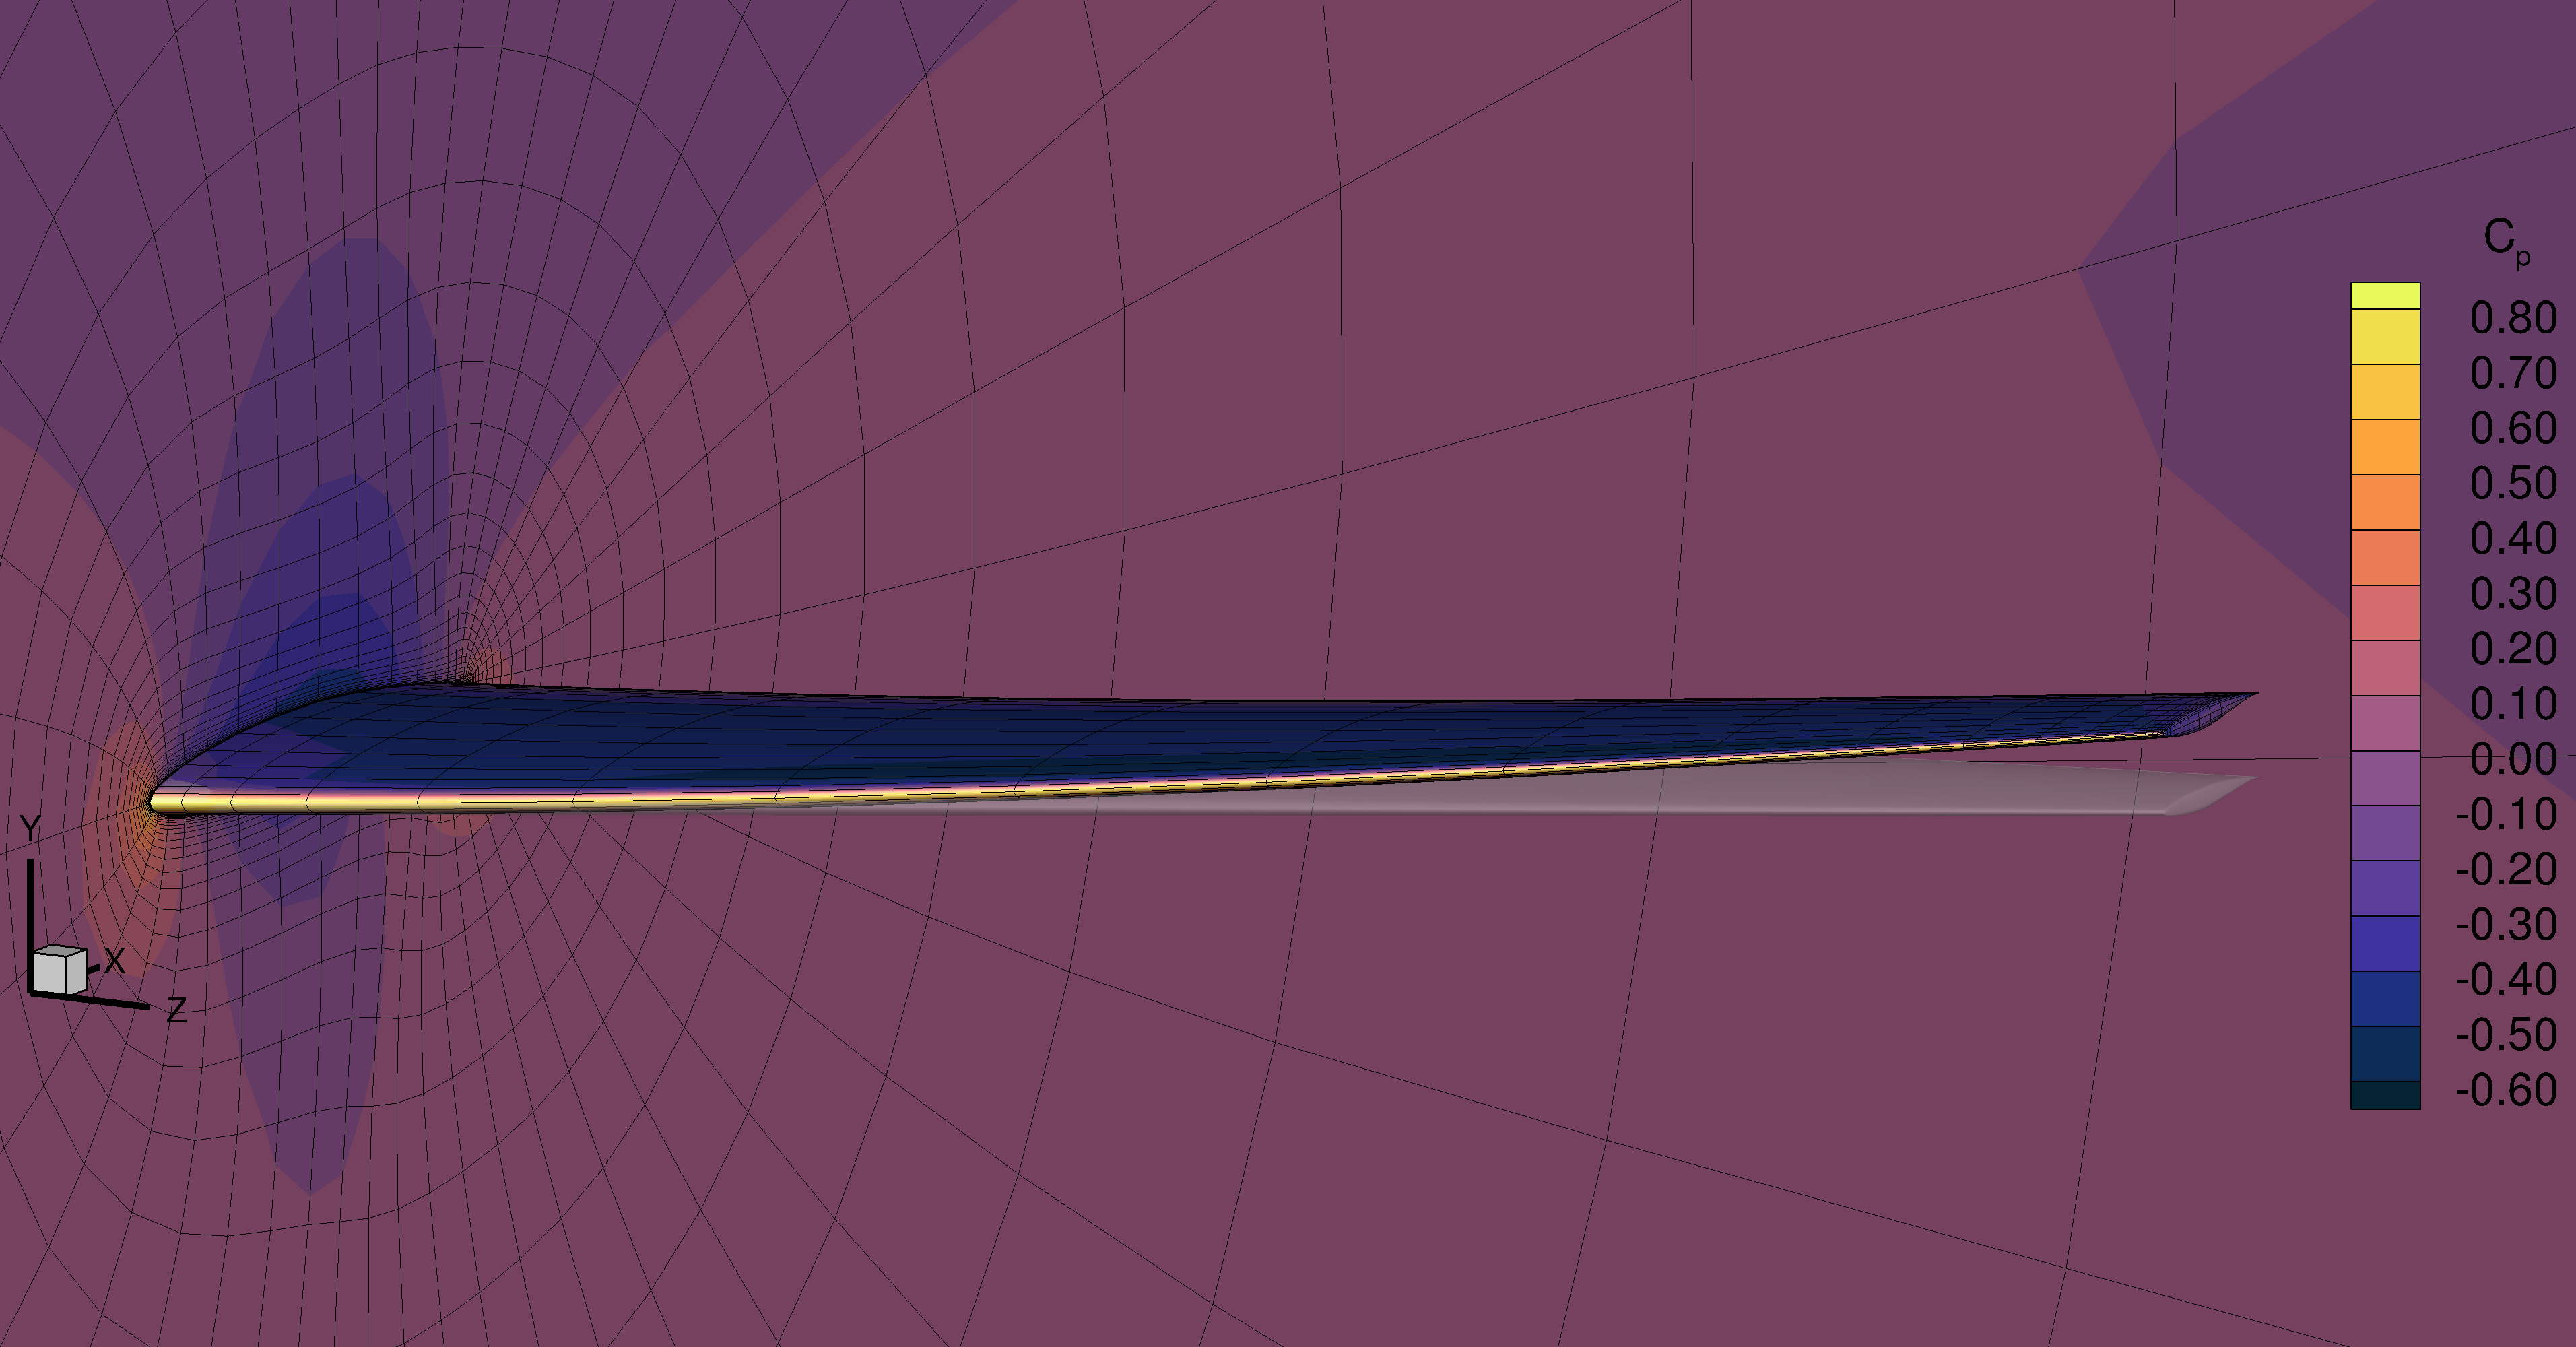
\includegraphics[width=1.05\linewidth]{images/aerostruct-resultDeformed.png} 
\caption{Results of a converged aerostructural analysis, with the undeformed shape shown in translucent gray while the updated, converged wing is shown as the resulting mesh with contours of coefficient of pressure.}
\end{figure}
\end{frame}
%---------------------------------------------------------------%

%---------------------------------------------------------------%
\begin{frame}{Discipline and Solver Coupling}
  eXtended Design Structure Matrix:
  \begin{figure}
    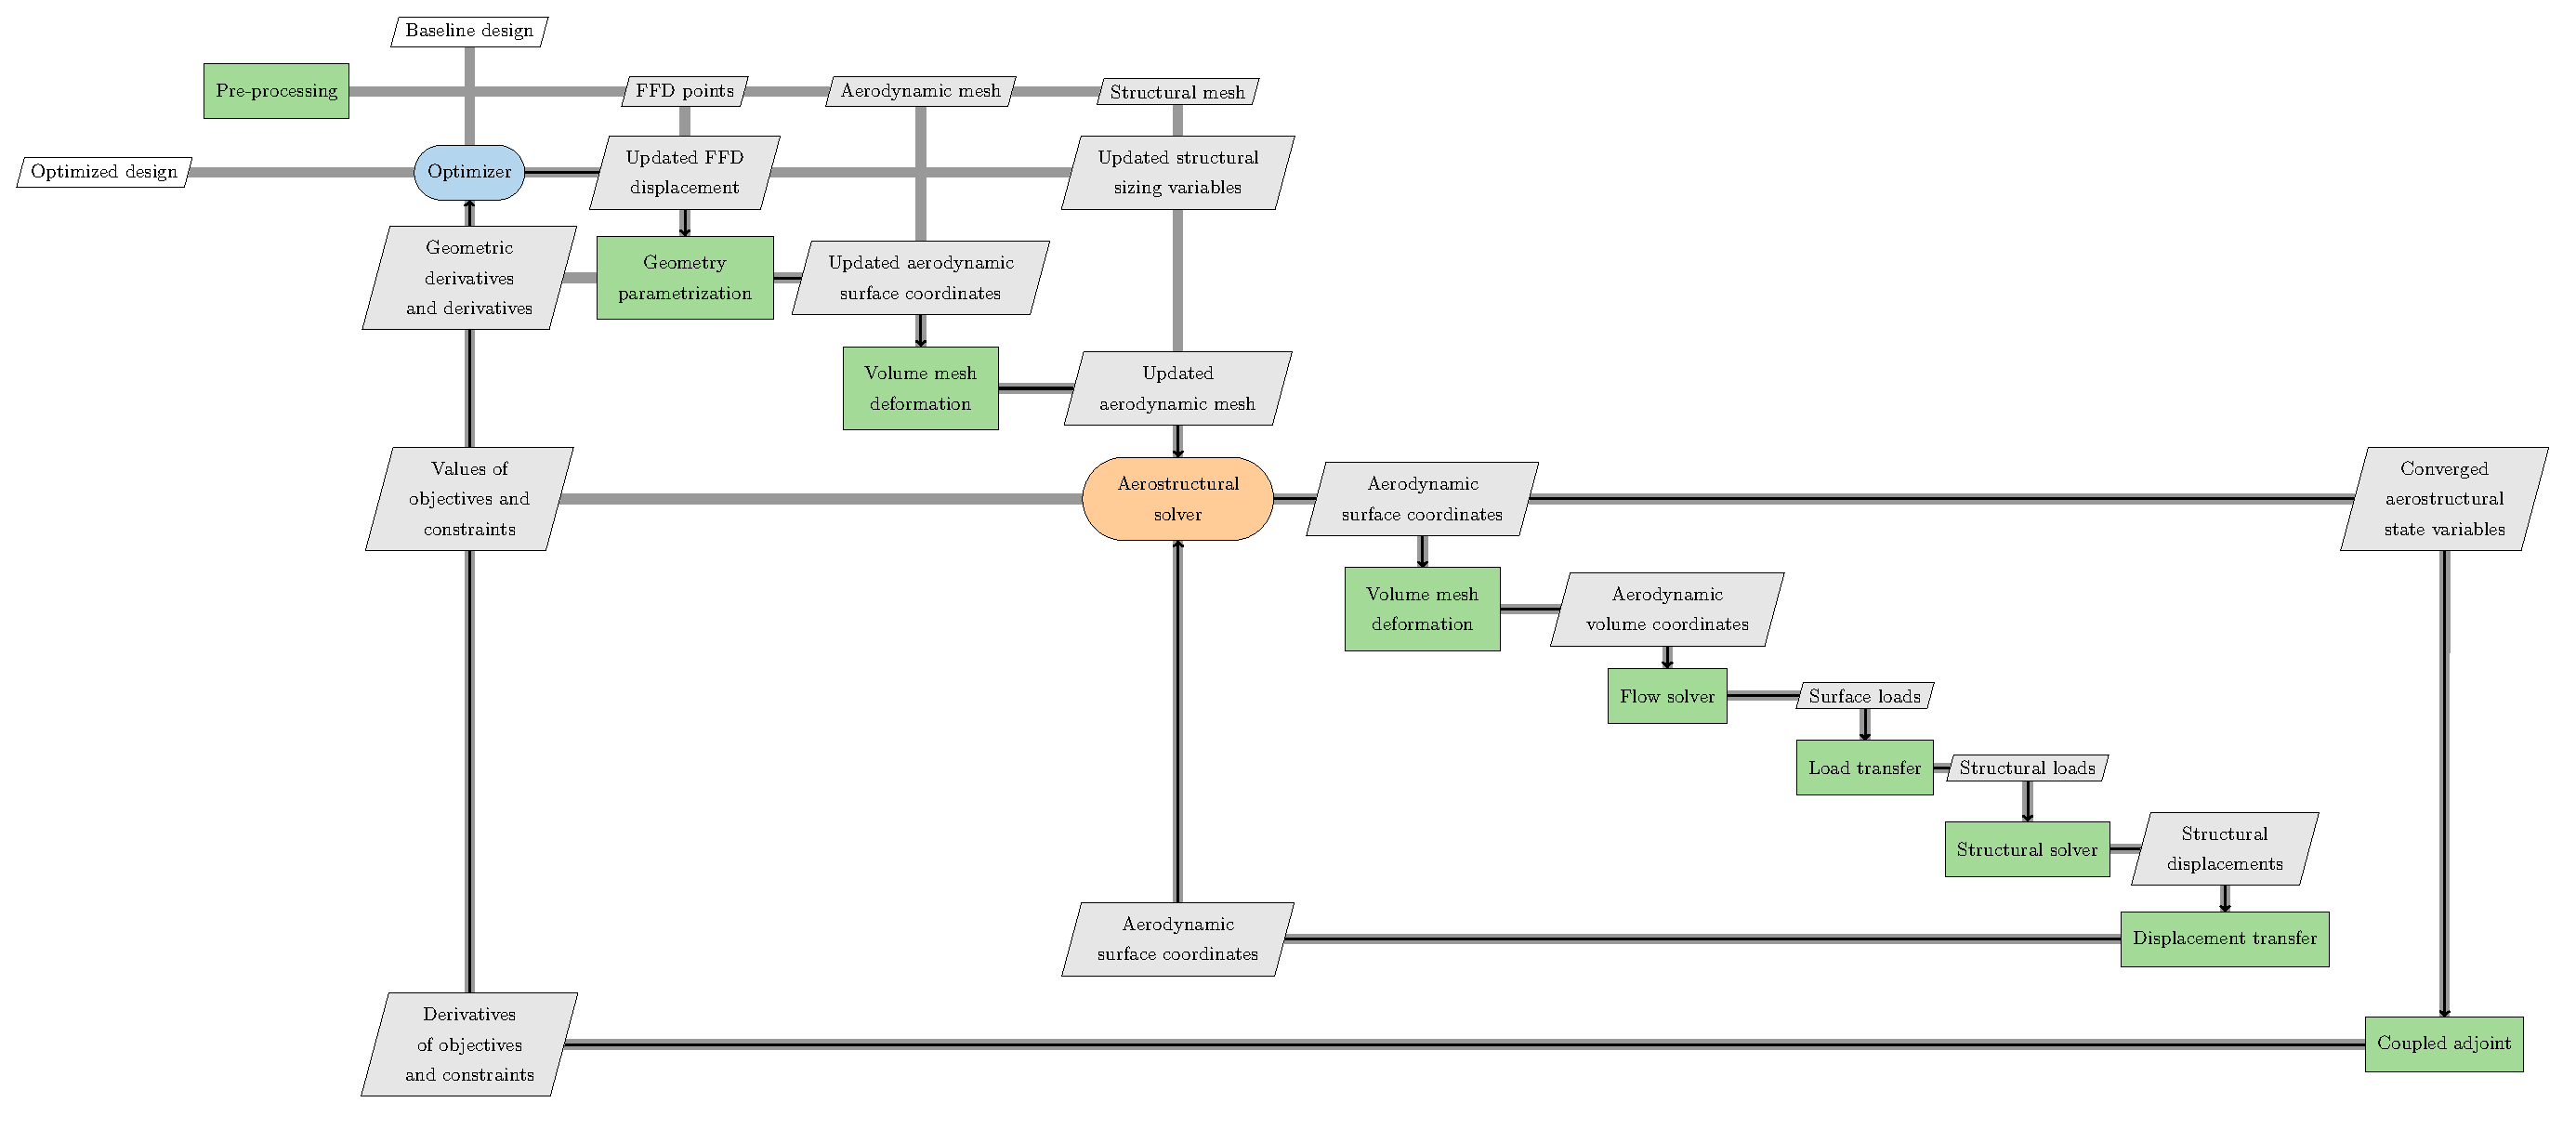
\includegraphics[width=1.0\linewidth]{images/aerostruct-xdsm.pdf} 
    \caption{Diagram for coupled aerostructural analysis and optimization. The diagonal elements specify computational blocks where green signifies analysis, yellow signifies solvers, and blue signifies the optimizer.}
  \end{figure}
\end{frame}
%---------------------------------------------------------------%

%---------------------------------------------------------------%
\begin{frame}[fragile]{Required Tools / Software}
  \begin{itemize}
    \setlength\itemsep{1em}
    \item The typical MACH packages required for aerodynamic optimization using DAFoam v3 (baseClasses, pySpline, pyGeo, IDWarp, DAFoam, pyOptSparse (optional), OpenMDAO, MPHYS)
    \item Matching-based Extrapolation for Load and Displacement transfer (MELD), needed for load and displacement transfer. Hosted within FUNtoFEM: \url{https://github.com/smdogroup/funtofem}
    \item Toolkit for the Analysis of Composite Structures (TACS), needed for finite element analysis: \url{https://github.com/smdogroup/tacs}
  \end{itemize}
\end{frame}
%---------------------------------------------------------------%

%---------------------------------------------------------------%
\begin{frame}{Problem Setup}
  \begin{columns}
    \begin{column}{0.5\textwidth}
      \begin{center}
        Aerodynamic Setup
      \end{center}
      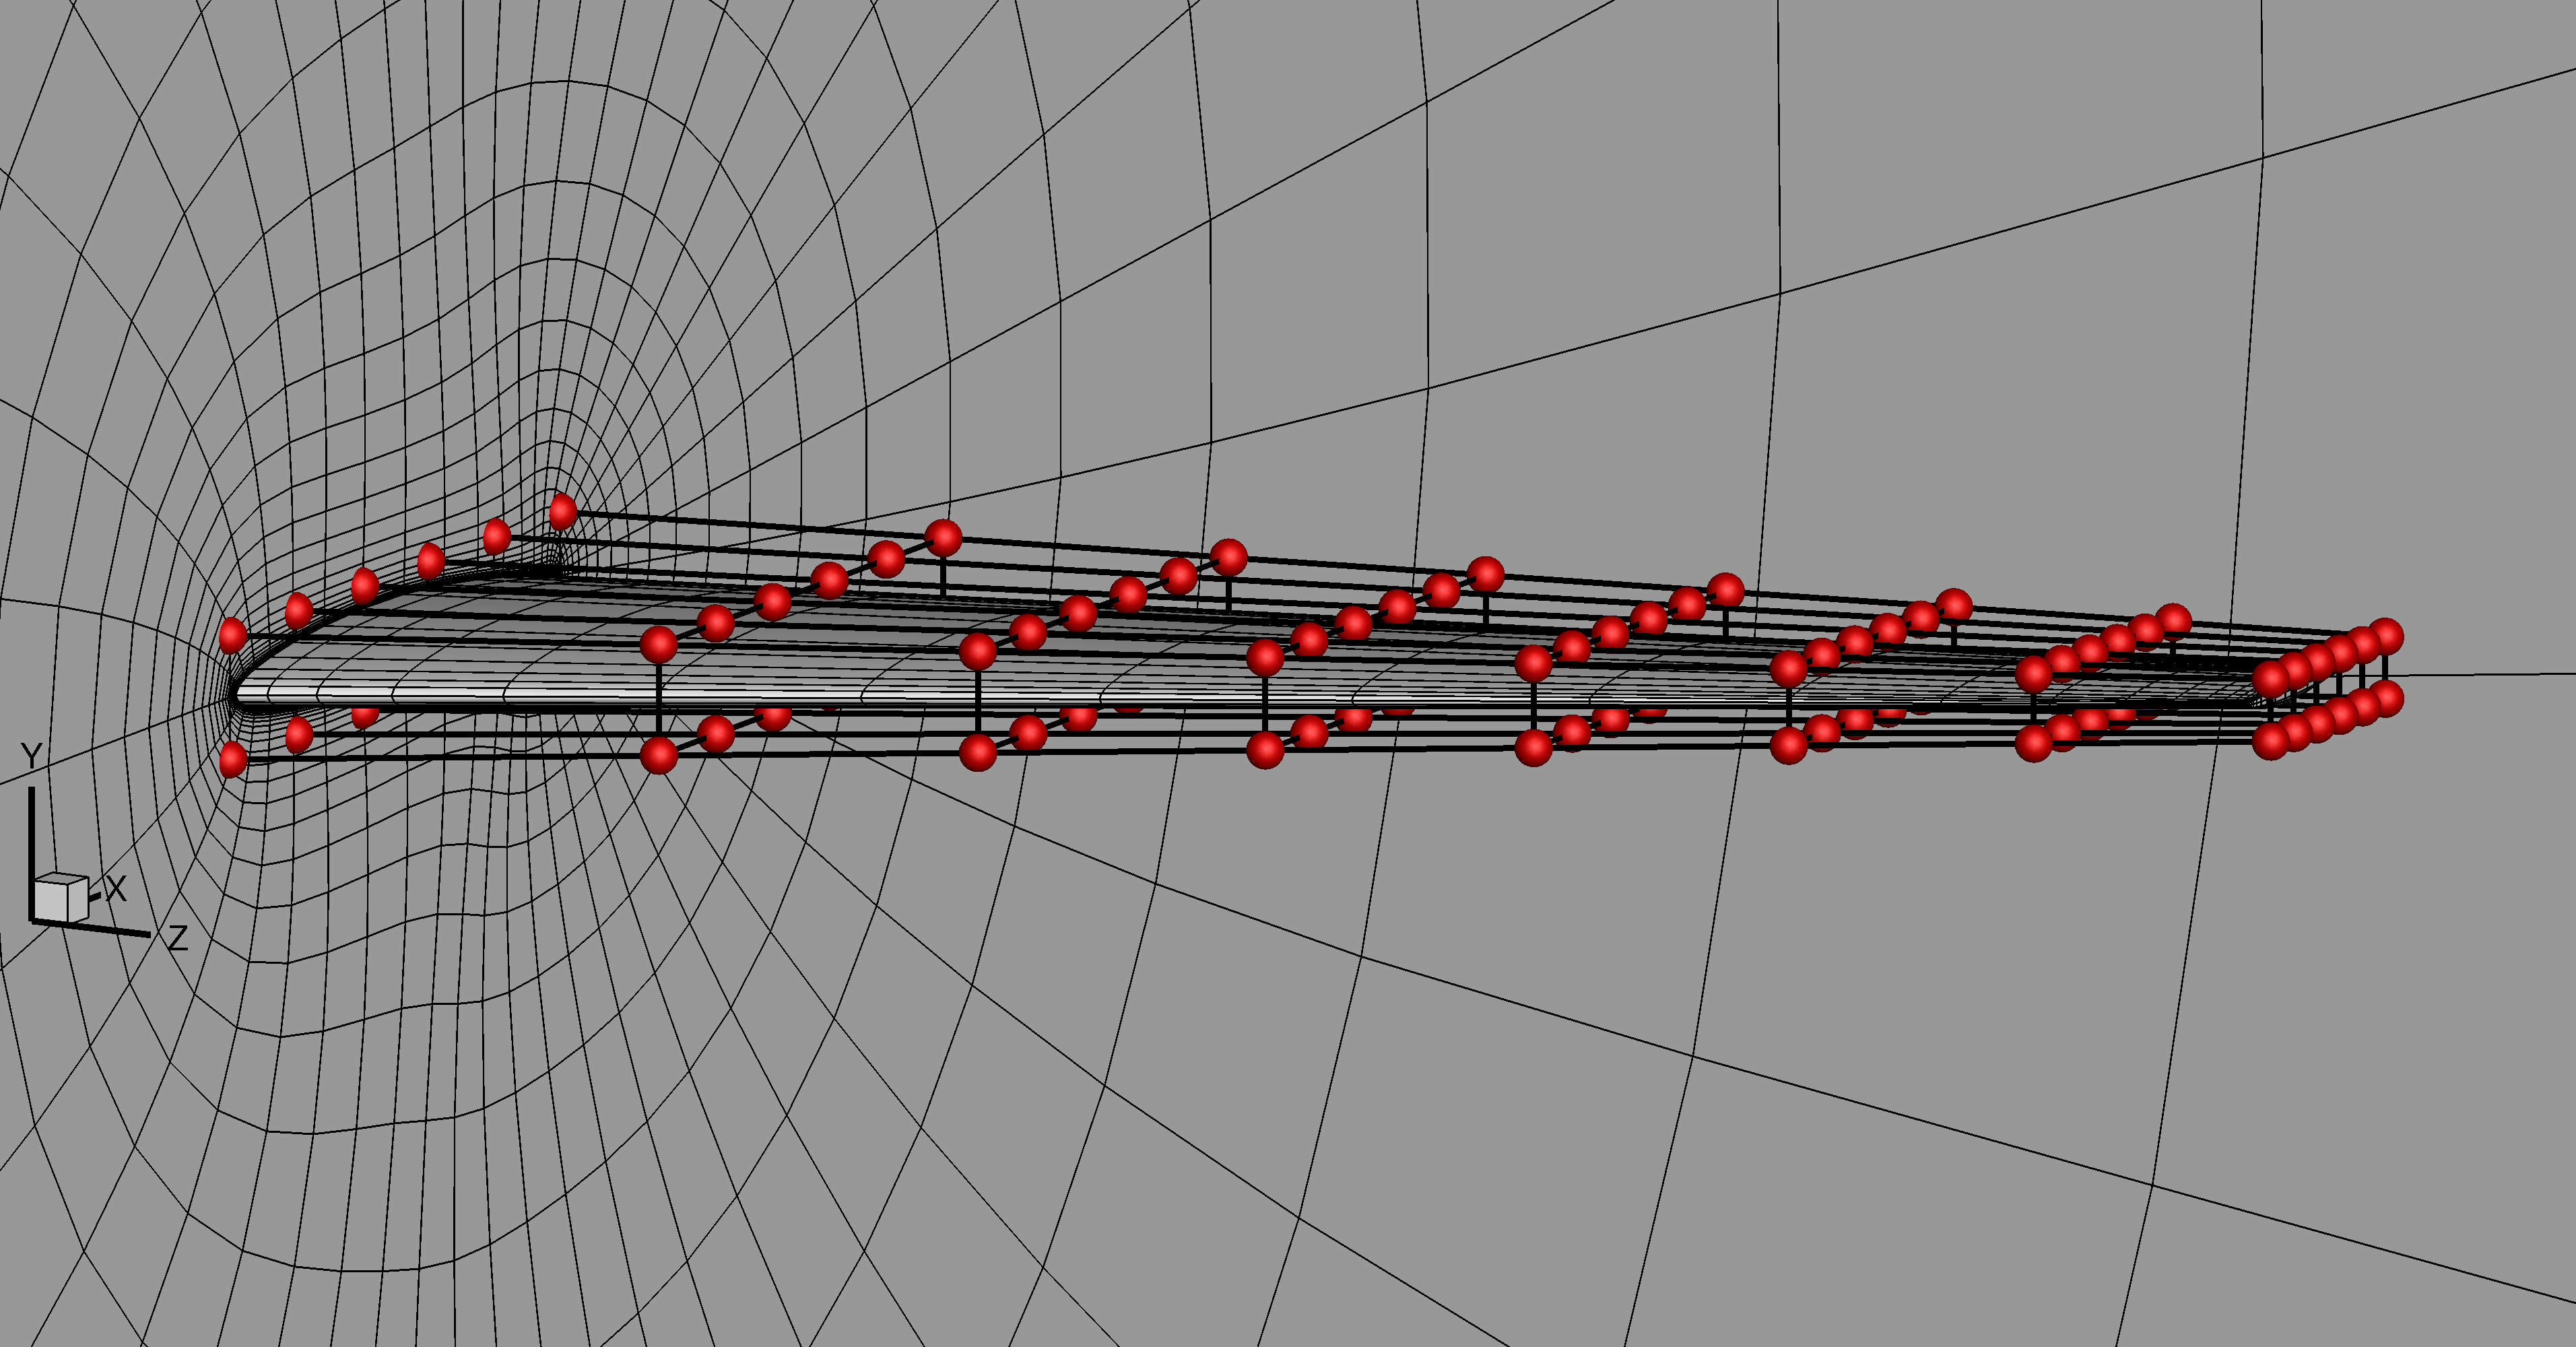
\includegraphics[width=1.0\linewidth]{images/aerostruct-aeroMeshFFD.png}
    \end{column}
    \begin{column}{0.5\textwidth}
      \begin{center}
        Structural Setup
      \end{center}
      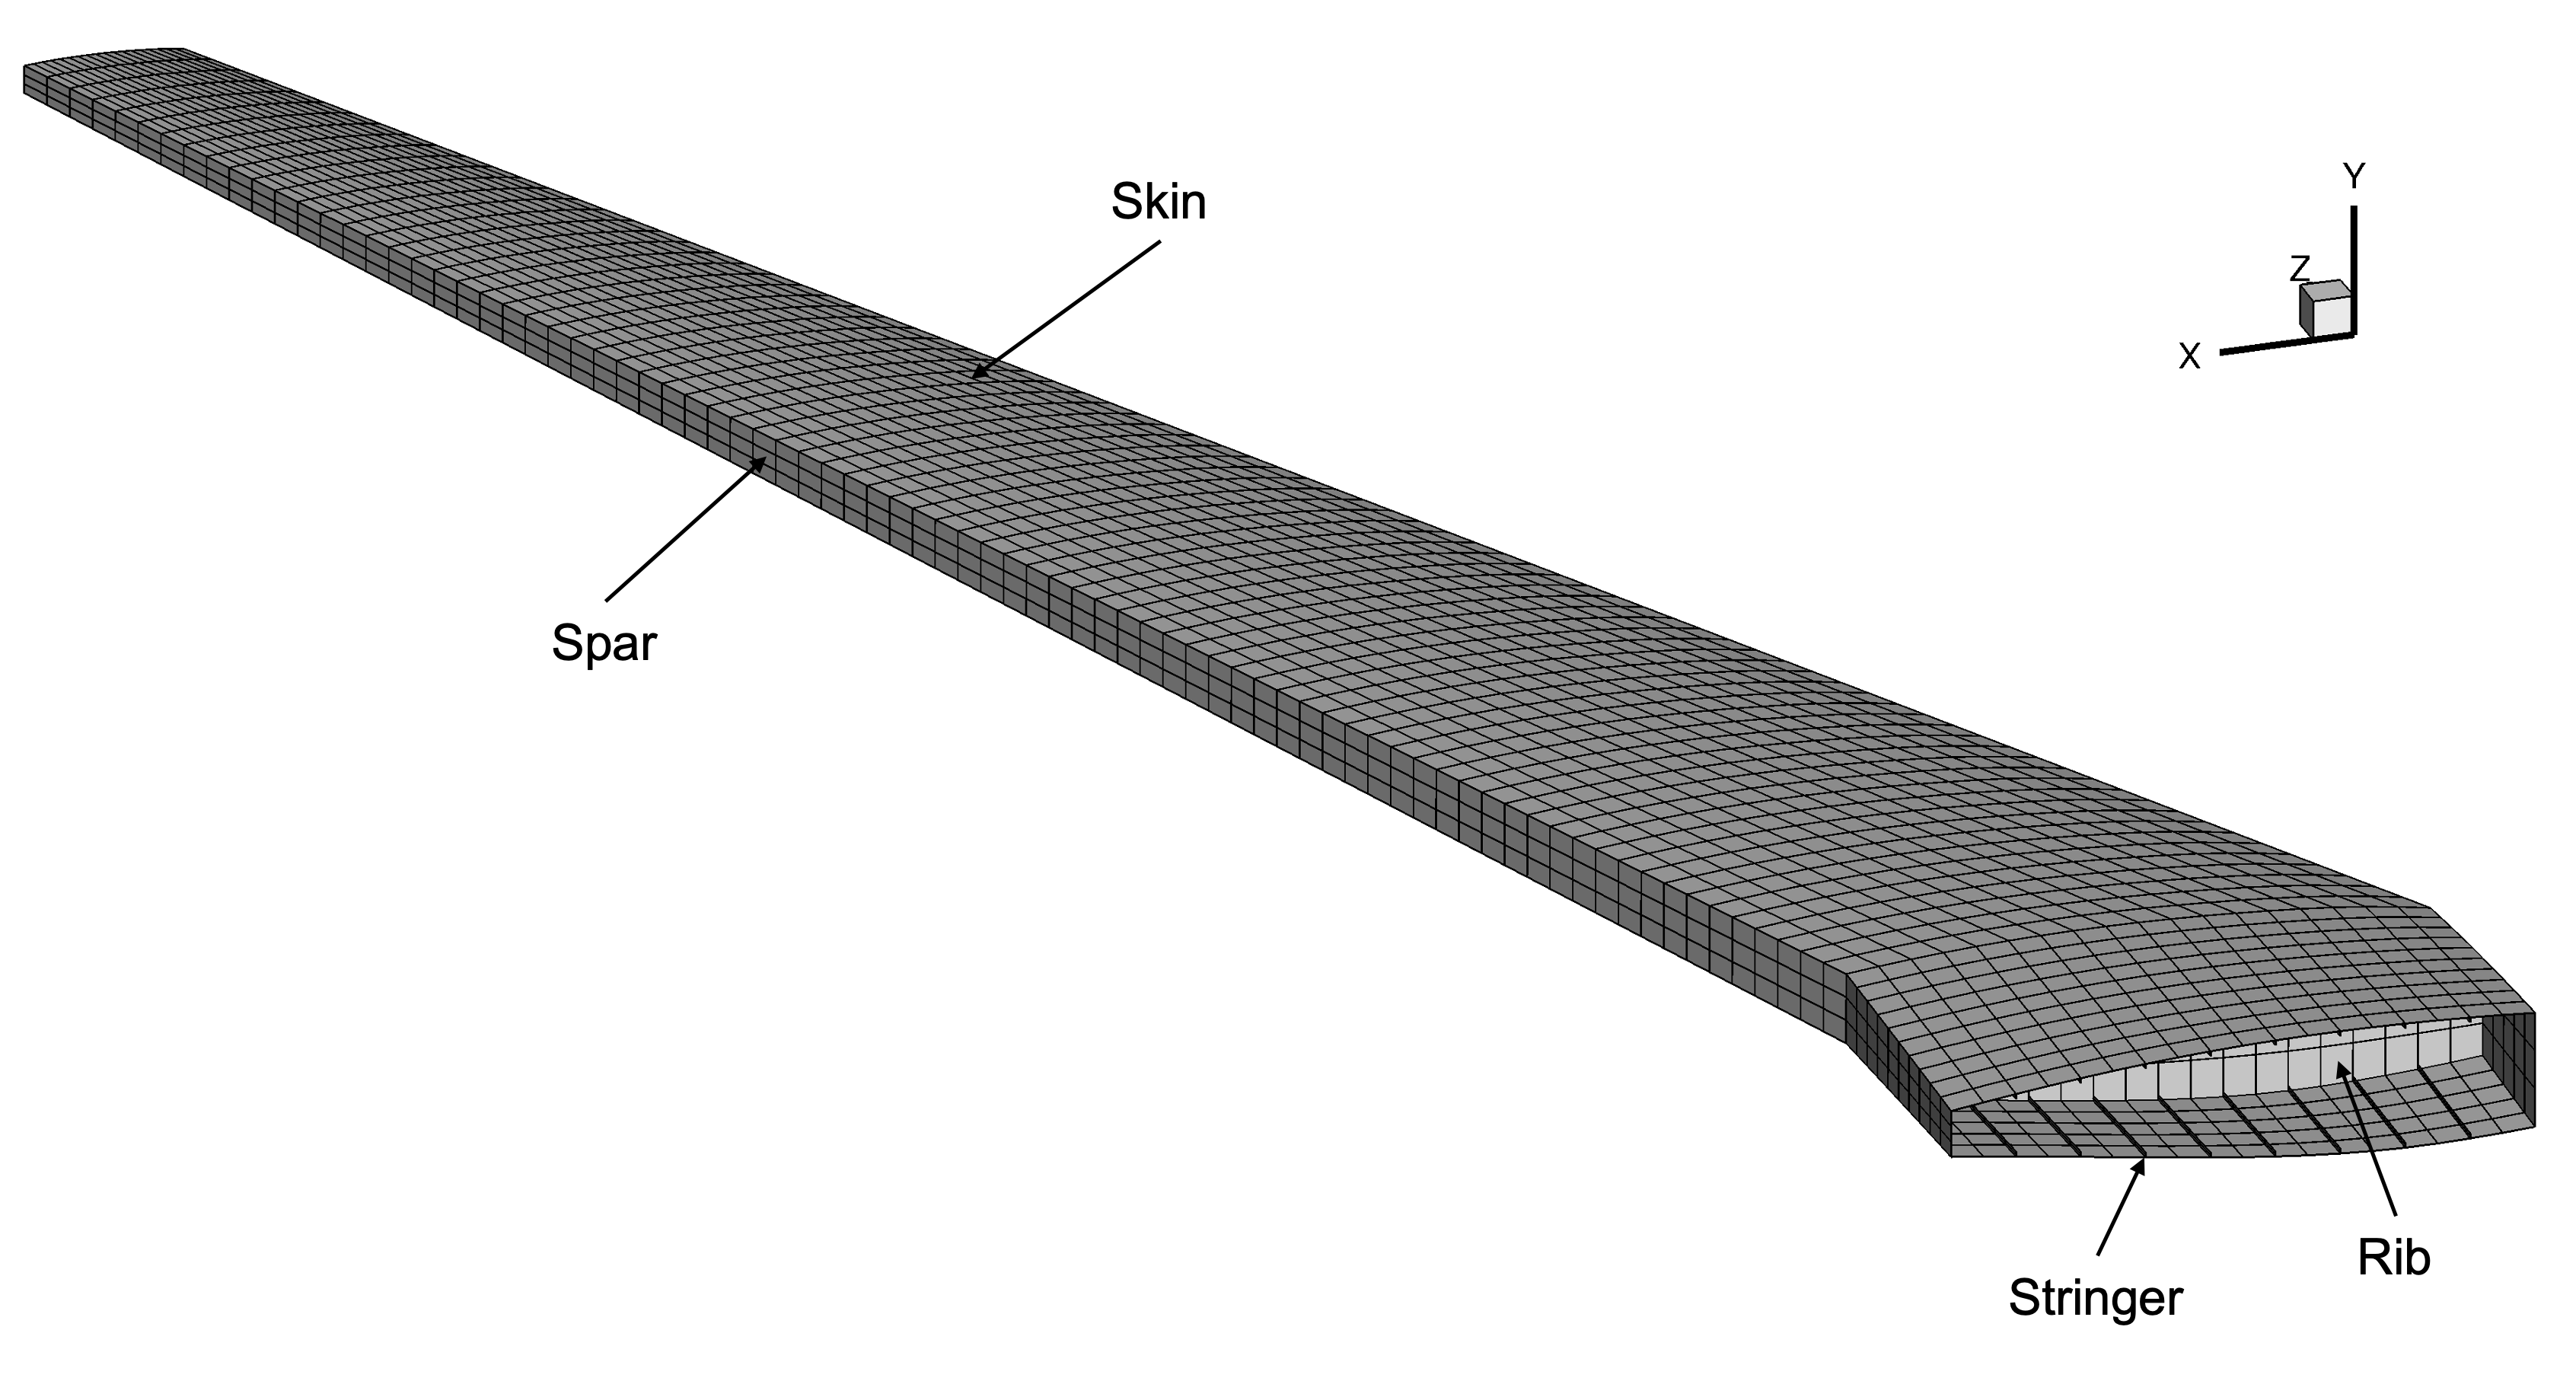
\includegraphics[width=1.0\linewidth]{images/aerostruct-structSetup.png}
    \end{column}
  \end{columns}
  \begin{itemize}
    \item \small The aerodyamic mesh and FFD are no different than a typical aerodynamic optimization case setup.
    \item \small The structural mesh consists of a finite element wingbox structure, with shell elements representing the ribs, spars, stringers, and skins.
    \item \small The aerodynamic and structural meshes should be constructed to correspond in the global coordinate frame of the optimization.
  \end{itemize}
\end{frame}
%---------------------------------------------------------------%

%---------------------------------------------------------------%
\begin{frame}{Summary of the aerostructural optimization case}

  \begin{table}
    \renewcommand{\arraystretch}{1.5}
    \small
    \centering
    \label{tab:implemented_models}
    \begin{tabular}{llllllllllll}
    \hline
    Optimizer   & SLSQP \\
    Flow and adjoint solvers  & DARhoSimpleFoam  \\
    Geometry  & MACH Tutorial Wing \\
    Objective function  & $C_D$ \\
    Design variables &7 twist, 96 FFDs, and $\alpha$ \\
    Constraint & \makecell[l]{$C_L=0.3$, Von Mises stress failure, thickness,\\volume, TE/LE}\\
    $U_\infty$  & 100 m/s \\
    Turbulence Model  & Spalart--Allmaras\\
     \hline
    \end{tabular}
  \end{table}

  You can find the case settings in workshops/2022\_Summer/examples/aerostructural.
\end{frame}
%---------------------------------------------------------------%

%---------------------------------------------------------------%
\begin{frame}[fragile]{runScript.py Details (1/21) - \large Package Imports}
The required packages are similar to the ones needed for aerodynamic analysis, with the addition of the load and displacement transfer tool (MELD) and the finite element analysis code (TACS).
\scriptsize
\lstset{ language=bash }
\begin{lstlisting}
import os
import argparse
import numpy as np
from mpi4py import MPI
import openmdao.api as om
from mphys.multipoint import Multipoint
from dafoam.mphys import DAFoamBuilder, OptFuncs
from tacs.mphys import TacsBuilder
from mphys.solver_builders.mphys_meld import MeldBuilder
from mphys.scenario_aerostructural import ScenarioAeroStructural
from pygeo.mphys import OM_DVGEOCOMP
from pygeo import geo_utils

parser = argparse.ArgumentParser()
# which optimizer to use. Options are: IPOPT (default), SLSQP, and SNOPT
parser.add_argument("-optimizer", help="optimizer to use", type=str, default="IPOPT")
# which task to run. Options are: opt (default), runPrimal, runAdjoint, checkTotals
parser.add_argument("-task", help="type of run to do", type=str, default="opt")
args = parser.parse_args()
\end{lstlisting}
\normalsize
\end{frame}
%---------------------------------------------------------------%

%---------------------------------------------------------------%
\begin{frame}[fragile]{runScript.py Details (2/21) - \large DAFoam Solver Settings}
The DAFoam solver options remain unchanged, except for the addition of a pressure correction term.
\scriptsize
\lstset{ language=bash }
\begin{lstlisting}
U0 = 100.0
p0 = 101325.0
nuTilda0 = 4.5e-5
T0 = 300.0
CL_target = 0.5
aoa0 = 2.0
rho0 = p0 / T0 / 287.0
A0 = 45.5

daOptions = {
  "designSurfaces": ["wing"],
  "solverName": "DARhoSimpleFoam",
  "primalMinResTol": 1.0e-8,
  "fsi": {"pRef": p0},  # set the ref pressure for computing force for FSI
  "primalBC": {
    "U0": {"variable": "U", "patches": ["inout"], "value": [U0, 0.0, 0.0]},
    "p0": {"variable": "p", "patches": ["inout"], "value": [p0]},
    "T0": {"variable": "T", "patches": ["inout"], "value": [T0]},
    "nuTilda0": {"variable": "nuTilda", "patches": ["inout"], "value": [nuTilda0]},
    "useWallFunction": True,
  },
\end{lstlisting}
\normalsize
\end{frame}
%---------------------------------------------------------------%

%---------------------------------------------------------------%
\begin{frame}[fragile]{runScript.py Details (3/21) - \large DAFoam Objective Functions}
Define the aerodynamic functions of interest in the same way as for the aerodynamic optimization case.
\scriptsize
\lstset{ language=bash }
\begin{lstlisting}
"objFunc": {
  "CD": {
    "part1": {
      "type": "force",
      "source": "patchToFace",
      "patches": ["wing"],
      "directionMode": "parallelToFlow",
      "alphaName": "aoa",
      "scale": 1.0 / (0.5 * U0 * U0 * A0 * rho0),
      "addToAdjoint": True,
    }
  },
  "CL": {
    "part1": {
      "type": "force",
      "source": "patchToFace",
      "patches": ["wing"],
      "directionMode": "normalToFlow",
      "alphaName": "aoa",
      "scale": 1.0 / (0.5 * U0 * U0 * A0 * rho0),
      "addToAdjoint": True,
    }
  },
},
\end{lstlisting}
\normalsize
\end{frame}
%---------------------------------------------------------------%

%---------------------------------------------------------------%
\begin{frame}[fragile]{runScript.py Details (4/21) - \large DAFoam Adjoint Settings}
When setting the adjoint options, consider that the DAFoam adjoint will be solved repeatedly when solving for coupled derivatives. Use a loose relative tolerance that will slowly converge to a much tighter absolute tolerance with each coupled iteration.
\scriptsize
\lstset{ language=bash }
\begin{lstlisting}
"adjEqnOption": {
  "gmresRelTol": 1.0e-2,  # set relative tolerance for block Gauss-Seidel adjoint
  "pcFillLevel": 1,
  "jacMatReOrdering": "rcm",
  "useNonZeroInitGuess": True,
},
"normalizeStates": {
  "U": U0,
  "p": p0,
  "T": T0,
  "nuTilda": 1e-3,
  "phi": 1.0,
},
\end{lstlisting}
\normalsize
\end{frame}
%---------------------------------------------------------------%

%---------------------------------------------------------------%
\begin{frame}[fragile]{runScript.py Details (5/21) - \large DAFoam CheckMesh Settings}
Aerostructural analysis and optimization require significant mesh deformation, both when updating the design itself and when displacing the geometry under load. In some cases, relax the mesh check thresholds to give DAFoam more flexibility when deforming the design.
\scriptsize
\lstset{ language=bash }
\begin{lstlisting}
"checkMeshThreshold": {
  "maxAspectRatio": 1000.0,
  "maxNonOrth": 70.0,
  "maxSkewness": 5.0,
},
\end{lstlisting}
\normalsize
\end{frame}
%---------------------------------------------------------------%

%---------------------------------------------------------------%
\begin{frame}[fragile]{runScript.py Details (6/21) - \large DAFoam Design Variables}
When using MPHYS and OpenMDAO, all of the DAFoam design variables \textit{must} be defined in the design variable dictionary. Otherwise, they may not be properly included in the problem setup.
\scriptsize
\lstset{ language=bash }
\begin{lstlisting}
"designVar": {
  "aoa": {"designVarType": "AOA", "patches": ["inout"], "flowAxis": "x", "normalAxis": "y"},
  "twist": {"designVarType": "FFD"},
  "shape": {"designVarType": "FFD"},
},
\end{lstlisting}
\normalsize
\end{frame}
%---------------------------------------------------------------%

%---------------------------------------------------------------%
\begin{frame}[fragile]{runScript.py Details (7/21) - \large Mesh Settings}
Finalize the DAFoam mesh setup as is done for the aerodynamic analysis case.

\vspace{0.25cm}

Import the TACS setup file and specify the finite element mesh to begin configuring the structural solver.
\scriptsize
\lstset{ language=bash }
\begin{lstlisting}
# Mesh deformation setup
meshOptions = {
  "gridFile": os.getcwd(),
  "fileType": "OpenFOAM",
  # point and normal for the symmetry plane
  "symmetryPlanes": [[[0.0, 0.0, 0.0], [0.0, 0.0, 1.0]]],
}

# TACS Setup
import tacsSetup
tacsOptions = {
    "element_callback": tacsSetup.element_callback,
    "problem_setup": tacsSetup.problem_setup,
    "mesh_file": "./wingbox.bdf",
}
\end{lstlisting}
\normalsize
\end{frame}
%---------------------------------------------------------------%

%---------------------------------------------------------------%
\begin{frame}[fragile]{runScript.py Details (8/21) - \large TACS Setup}
\textcolor{red}{\textit{This file is separate from the runscript and is used to specify the TACS setup.}}

\vspace{0.25cm}

Import the TACS packages and define the material and element properties.

\scriptsize
\lstset{ language=bash }
\begin{lstlisting}
import numpy as np
from tacs import elements, constitutive, functions

# Material properties
rho = 2780.0  # density, kg/m^3
E = 73.1e9  # elastic modulus, Pa
nu = 0.33  # poisson's ratio
kcorr = 5.0 / 6.0  # shear correction factor
ys = 324.0e6  # yield stress, Pa

# Shell thickness
t = 0.003  # m
tMin = 0.002  # m
tMax = 0.05  # m
\end{lstlisting}
\normalsize
\end{frame}
%---------------------------------------------------------------%

%---------------------------------------------------------------%
\begin{frame}[fragile]{runScript.py Details (9/21) - \large TACS Element Function}
\textcolor{red}{\textit{This file is separate from the runscript and is used to specify the TACS setup.}}

\vspace{0.25cm}

Define the element callback function, used in TACS to define the element type and properties.
\scriptsize
\lstset{ language=bash }
\begin{lstlisting}
def element_callback(dvNum, compID, compDescript, elemDescripts, specialDVs, **kwargs):
  # Setup (isotropic) property and constitutive objects
  prop = constitutive.MaterialProperties(rho=rho, E=E, nu=nu, ys=ys)
  # Set one thickness dv for every component
  con = constitutive.IsoShellConstitutive(prop, t=t, tNum=dvNum, tlb=tMin, tub=tMax)

  # For each element type in this component,
  # pass back the appropriate tacs element object
  transform = None
  elem = elements.Quad4Shell(transform, con)

  return elem
\end{lstlisting}
\normalsize
\end{frame}
%---------------------------------------------------------------%

%---------------------------------------------------------------%
\begin{frame}[fragile]{runScript.py Details (10/21) - \large TACS Problem Setup}
\textcolor{red}{\textit{This file is separate from the runscript and is used to specify the TACS setup.}}

\vspace{0.25cm}

Set up the TACS problem, defining the functions of interest and any additional structural loads.

\scriptsize
\lstset{ language=bash }
\begin{lstlisting}
def problem_setup(scenario_name, fea_assembler, problem):
  """
  Helper function to add fixed forces and eval functions
  to structural problems used in tacs builder
  """
  # Add TACS Functions
  # Only include mass from elements that belong to pytacs components (i.e. skip concentrated masses)
  problem.addFunction("mass", functions.StructuralMass)
  problem.addFunction("ks_vmfailure", functions.KSFailure, safetyFactor=1.0, ksWeight=50.0)

  # Add gravity load
  g = np.array([0.0, 0.0, -9.81])  # m/s^2
  problem.addInertialLoad(g)
\end{lstlisting}
\normalsize
\end{frame}
%---------------------------------------------------------------%

%---------------------------------------------------------------%
\begin{frame}[fragile]{runScript.py Details (11/21) - \large Solver Setup}

Set up the MPHYS components by defining the solvers: DAFoam (aerodynamic analysis), TACS (structural analysis), and MELD (load and displacement transfer).

\scriptsize
\lstset{ language=bash }
\begin{lstlisting}
class Top(Multipoint):
  def setup(self):
    # create the builder to initialize the DASolvers
    aero_builder = DAFoamBuilder(daOptions, meshOptions, scenario="aerostructural")
    aero_builder.initialize(self.comm)

    # add the aerodynamic mesh component
    self.add_subsystem("mesh_aero", aero_builder.get_mesh_coordinate_subsystem())

    # create the builder to initialize TACS
    struct_builder = TacsBuilder(tacsOptions)
    struct_builder.initialize(self.comm)

    # add the structure mesh component
    self.add_subsystem("mesh_struct", struct_builder.get_mesh_coordinate_subsystem())

    # load and displacement transfer builder (meld), isym sets the symmetry plan axis (k)
    xfer_builder = MeldBuilder(aero_builder, struct_builder, isym=2, check_partials=True)
    xfer_builder.initialize(self.comm)
\end{lstlisting}
\normalsize
\end{frame}
%---------------------------------------------------------------%

%---------------------------------------------------------------%
\begin{frame}[fragile]{runScript.py Details (12/21) - \large Scenario Setup}

Define the design variable component and geometry handler, as well as the aerostructural solvers and MPHYS scenario. The initialized solvers are responsible for converging the aerostructural analysis blocks. The scenario combines all of the solvers to configure the aerostructural problem.
\scriptsize
\lstset{ language=bash }
\begin{lstlisting}
# add the design variable component to keep the top level design variables
dvs = self.add_subsystem("dvs", om.IndepVarComp(), promotes=["*"])

# add the geometry component (FFD)
self.add_subsystem("geometry", OM_DVGEOCOMP(ffd_file="FFD/wingFFD.xyz"))

# primal and adjoint solution options, i.e., nonlinear block Gauss-Seidel for aerostructural analysis
# and linear block Gauss-Seidel for the coupled adjoint
nonlinear_solver = om.NonlinearBlockGS(maxiter=25, iprint=2, use_aitken=True, rtol=1e-8, atol=1e-8)
linear_solver = om.LinearBlockGS(maxiter=25, iprint=2, use_aitken=True, rtol=1e-6, atol=1e-6)
# add the coupling aerostructural scenario
self.mphys_add_scenario(
  "cruise",
  ScenarioAeroStructural(
    aero_builder=aero_builder, struct_builder=struct_builder, ldxfer_builder=xfer_builder
  ),
  nonlinear_solver,
  linear_solver,
)
\end{lstlisting}
\normalsize
\end{frame}
%---------------------------------------------------------------%

%---------------------------------------------------------------%
\begin{frame}[fragile]{runScript.py Details (13/21) - \large Aerostructural Connections}
Connect the aerodynamic and structural design variables to ensure the required data is provided to all components.
\scriptsize
\lstset{ language=bash }
\begin{lstlisting}
# need to manually connect the vars in the geo component to cruise
for discipline in ["aero", "struct"]:
  self.connect("geometry.x_%s0" % discipline, "cruise.x_%s0" % discipline)

# add the structural thickness DVs
ndv_struct = struct_builder.get_ndv()
dvs.add_output("dv_struct", np.array(ndv_struct * [0.01]))
self.connect("dv_struct", "cruise.dv_struct")

# more manual connection
self.connect("mesh_aero.x_aero0", "geometry.x_aero_in")
self.connect("mesh_struct.x_struct0", "geometry.x_struct_in")
\end{lstlisting}
\normalsize
\end{frame}
%---------------------------------------------------------------%

%---------------------------------------------------------------%
\begin{frame}[fragile]{runScript.py Details (14/21) - \large Problem Configuration}
Configure the optimization problem, setting the functions of interest and retrieving the initialized computational meshes.

\scriptsize
\lstset{ language=bash }
\begin{lstlisting}
def configure(self):
  # call this to configure the coupling solver
  super().configure()

  # add the objective function to the cruise scenario
  self.cruise.aero_post.mphys_add_funcs()

  # get the surface coordinates from the mesh component
  points = self.mesh_aero.mphys_get_surface_mesh()

  # add pointset for both aero and struct
  self.geometry.nom_add_discipline_coords("aero", points)
  self.geometry.nom_add_discipline_coords("struct")

  # set the triangular points to the geometry component for geometric constraints
  tri_points = self.mesh_aero.mphys_get_triangulated_surface()
  self.geometry.nom_setConstraintSurface(tri_points)
\end{lstlisting}
\normalsize
\end{frame}
%---------------------------------------------------------------%

%---------------------------------------------------------------%
\begin{frame}[fragile]{runScript.py Details (15/21) - \large FFD Variable Definitions}
Define the FFD-based design variables in the same way as for the aerodynamic optimization case.
  \scriptsize
\lstset{ language=bash }
\begin{lstlisting}
# Create reference axis for the twist variable
nRefAxPts = self.geometry.nom_addRefAxis(name="wingAxis", xFraction=0.25, alignIndex="k")

# Set up global design variables. We dont change the root twist
def twist(val, geo):
  for i in range(1, nRefAxPts):
    geo.rot_z["wingAxis"].coef[i] = -val[i - 1]

# add twist variable
self.geometry.nom_addGeoDVGlobal(dvName="twist", value=np.array([0] * (nRefAxPts - 1)), func=twist)

# add shape variable
pts = self.geometry.DVGeo.getLocalIndex(0)
indexList = pts[:, :, :].flatten()
PS = geo_utils.PointSelect("list", indexList)
nShapes = self.geometry.nom_addGeoDVLocal(dvName="shape", pointSelect=PS)
\end{lstlisting}
\normalsize
\end{frame}
%---------------------------------------------------------------%

%---------------------------------------------------------------%
\begin{frame}[fragile]{runScript.py Details (16/21) - \large Angle of Attack Definition}
Define the angle of attack design variable in the same way as for the aerodynamic optimization case, and add it as a function in DAFoam.
\scriptsize
\lstset{ language=bash }
\begin{lstlisting}
# define an angle of attack function to change the U direction at the far field
def aoa(val, DASolver):
  aoa = val[0] * np.pi / 180.0
  U = [float(U0 * np.cos(aoa)), float(U0 * np.sin(aoa)), 0]
  # we need to update the U value only
  DASolver.setOption("primalBC", {"U0": {"value": U}})
  DASolver.updateDAOption()

# pass this aoa function to the cruise group
self.cruise.coupling.aero.solver.add_dv_func("aoa", aoa)
self.cruise.aero_post.add_dv_func("aoa", aoa)
\end{lstlisting}
\normalsize
\end{frame}
%---------------------------------------------------------------%

%---------------------------------------------------------------%
\begin{frame}[fragile]{runScript.py Details (17/21) - \large Geometric Constraints}
Configure the geometric constraints, for example leading edge / trailing edge constraints, thickness constraints, and volume constraints.
\scriptsize
\lstset{ language=bash }
\begin{lstlisting}
# setup the volume and thickness constraints
leList = [[0.1, 0, 0.01], [7.5, 0, 13.9]]
teList = [[4.9, 0, 0.01], [8.9, 0, 13.9]]
self.geometry.nom_addThicknessConstraints2D("thickcon", leList, teList, nSpan=10, nChord=10)
self.geometry.nom_addVolumeConstraint("volcon", leList, teList, nSpan=10, nChord=10)
# add the LE/TE constraints
self.geometry.nom_add_LETEConstraint("lecon", volID=0, faceID="iLow")
self.geometry.nom_add_LETEConstraint("tecon", volID=0, faceID="iHigh")
\end{lstlisting}
\normalsize
\end{frame}
%---------------------------------------------------------------%

%---------------------------------------------------------------%
\begin{frame}[fragile]{runScript.py Details (18/21) - \large Design Variables}
Initialize the design variables in OpenMDAO and connect them to the respective values in the optimization problem. Specify any bounds or variable scaling as desired.
\scriptsize
\lstset{ language=bash }
\begin{lstlisting}
# add the design variables to the dvs component's output
self.dvs.add_output("twist", val=np.array([0] * (nRefAxPts - 1)))
self.dvs.add_output("shape", val=np.array([0] * nShapes))
self.dvs.add_output("aoa", val=np.array([aoa0]))

# manually connect the dvs output to the geometry and cruise
self.connect("twist", "geometry.twist")
self.connect("shape", "geometry.shape")
self.connect("aoa", "cruise.aoa")

# define the design variables
self.add_design_var("twist", lower=-10.0, upper=10.0, scaler=1.0)
self.add_design_var("shape", lower=-1.0, upper=1.0, scaler=1.0)
self.add_design_var("aoa", lower=0.0, upper=10.0, scaler=1.0)
\end{lstlisting}
\normalsize
\end{frame}
%---------------------------------------------------------------%

%---------------------------------------------------------------%
\begin{frame}[fragile]{runScript.py Details (19/21) - \large Objective and Constraints}
Define the objective and constraint functions. Specify the lower / upper / equivalent values for constraints as well as any function scaling.
\scriptsize
\lstset{ language=bash }
\begin{lstlisting}
# add constraints and the objective
self.add_objective("cruise.aero_post.CD", scaler=1.0)
self.add_constraint("cruise.aero_post.CL", equals=0.3, scaler=1.0)
self.add_constraint("cruise.ks_vmfailure", lower=0.0, upper=1.0, scaler=1.0)
self.add_constraint("geometry.thickcon", lower=0.5, upper=3.0, scaler=1.0)
self.add_constraint("geometry.volcon", lower=1.0, scaler=1.0)
self.add_constraint("geometry.tecon", equals=0.0, scaler=1.0, linear=True)
self.add_constraint("geometry.lecon", equals=0.0, scaler=1.0, linear=True)
\end{lstlisting}
\normalsize
\end{frame}
%---------------------------------------------------------------%

%---------------------------------------------------------------%
\begin{frame}[fragile]{runScript.py Details (20/21) - \large Optimization Settings}
Finalize the OpenMDAO problem definition and specify the optimizer, along with its options.
\scriptsize
\lstset{ language=bash }
\begin{lstlisting}
# OpenMDAO setup
prob = om.Problem()
prob.model = Top()
prob.setup(mode="rev")
om.n2(prob, show_browser=False, outfile="mphys_aero_struct.html")

# initialize the optimization function
optFuncs = OptFuncs(daOptions, prob)

# use pyoptsparse to setup optimization
prob.driver = om.pyOptSparseDriver()
prob.driver.options["optimizer"] = args.optimizer

prob.driver.opt_settings = {
  "ACC": 1.0e-5,
  "MAXIT": 100,
  "IFILE": "opt_SLSQP.txt",
}

prob.driver.options["debug_print"] = ["nl_cons", "objs", "desvars"]
prob.driver.options["print_opt_prob"] = True
prob.driver.hist_file = "OptView.hst"

\end{lstlisting}
\normalsize
\end{frame}
%---------------------------------------------------------------%

%---------------------------------------------------------------%
\begin{frame}[fragile]{runScript.py Details (21/21) - \large Task Runner}
Run the case. Using the built in OpenMDAO features one can run the analysis, run the optimization, run the adjoint, or check the total derivatives.
\scriptsize
\lstset{ language=bash }
\begin{lstlisting}
if args.task == "opt":
  # solve CL
  optFuncs.findFeasibleDesign(["cruise.aero_post.CL"], ["aoa"], targets=[CL_target])
  # run the optimization
  prob.run_driver()
elif args.task == "runPrimal":
  # just run the primal once
  prob.run_model()
elif args.task == "runAdjoint":
  # just run the primal and adjoint once
  prob.run_model()
  totals = prob.compute_totals()
  if MPI.COMM_WORLD.rank == 0:
      print(totals)
elif args.task == "checkTotals":
  # verify the total derivatives against the finite-difference
  prob.run_model()
  prob.check_totals(
    of=["CD", "CL"], wrt=["shape", "aoa"], compact_print=True, step=1e-3, form="central", step_calc="abs"
  )
else:
  print("task arg not found!")
  exit(1)
\end{lstlisting}
\normalsize
\end{frame}
%---------------------------------------------------------------%

%---------------------------------------------------------------%
\begin{frame}{OpenMDAO Representation - N2 Diagram}
  \begin{figure}
  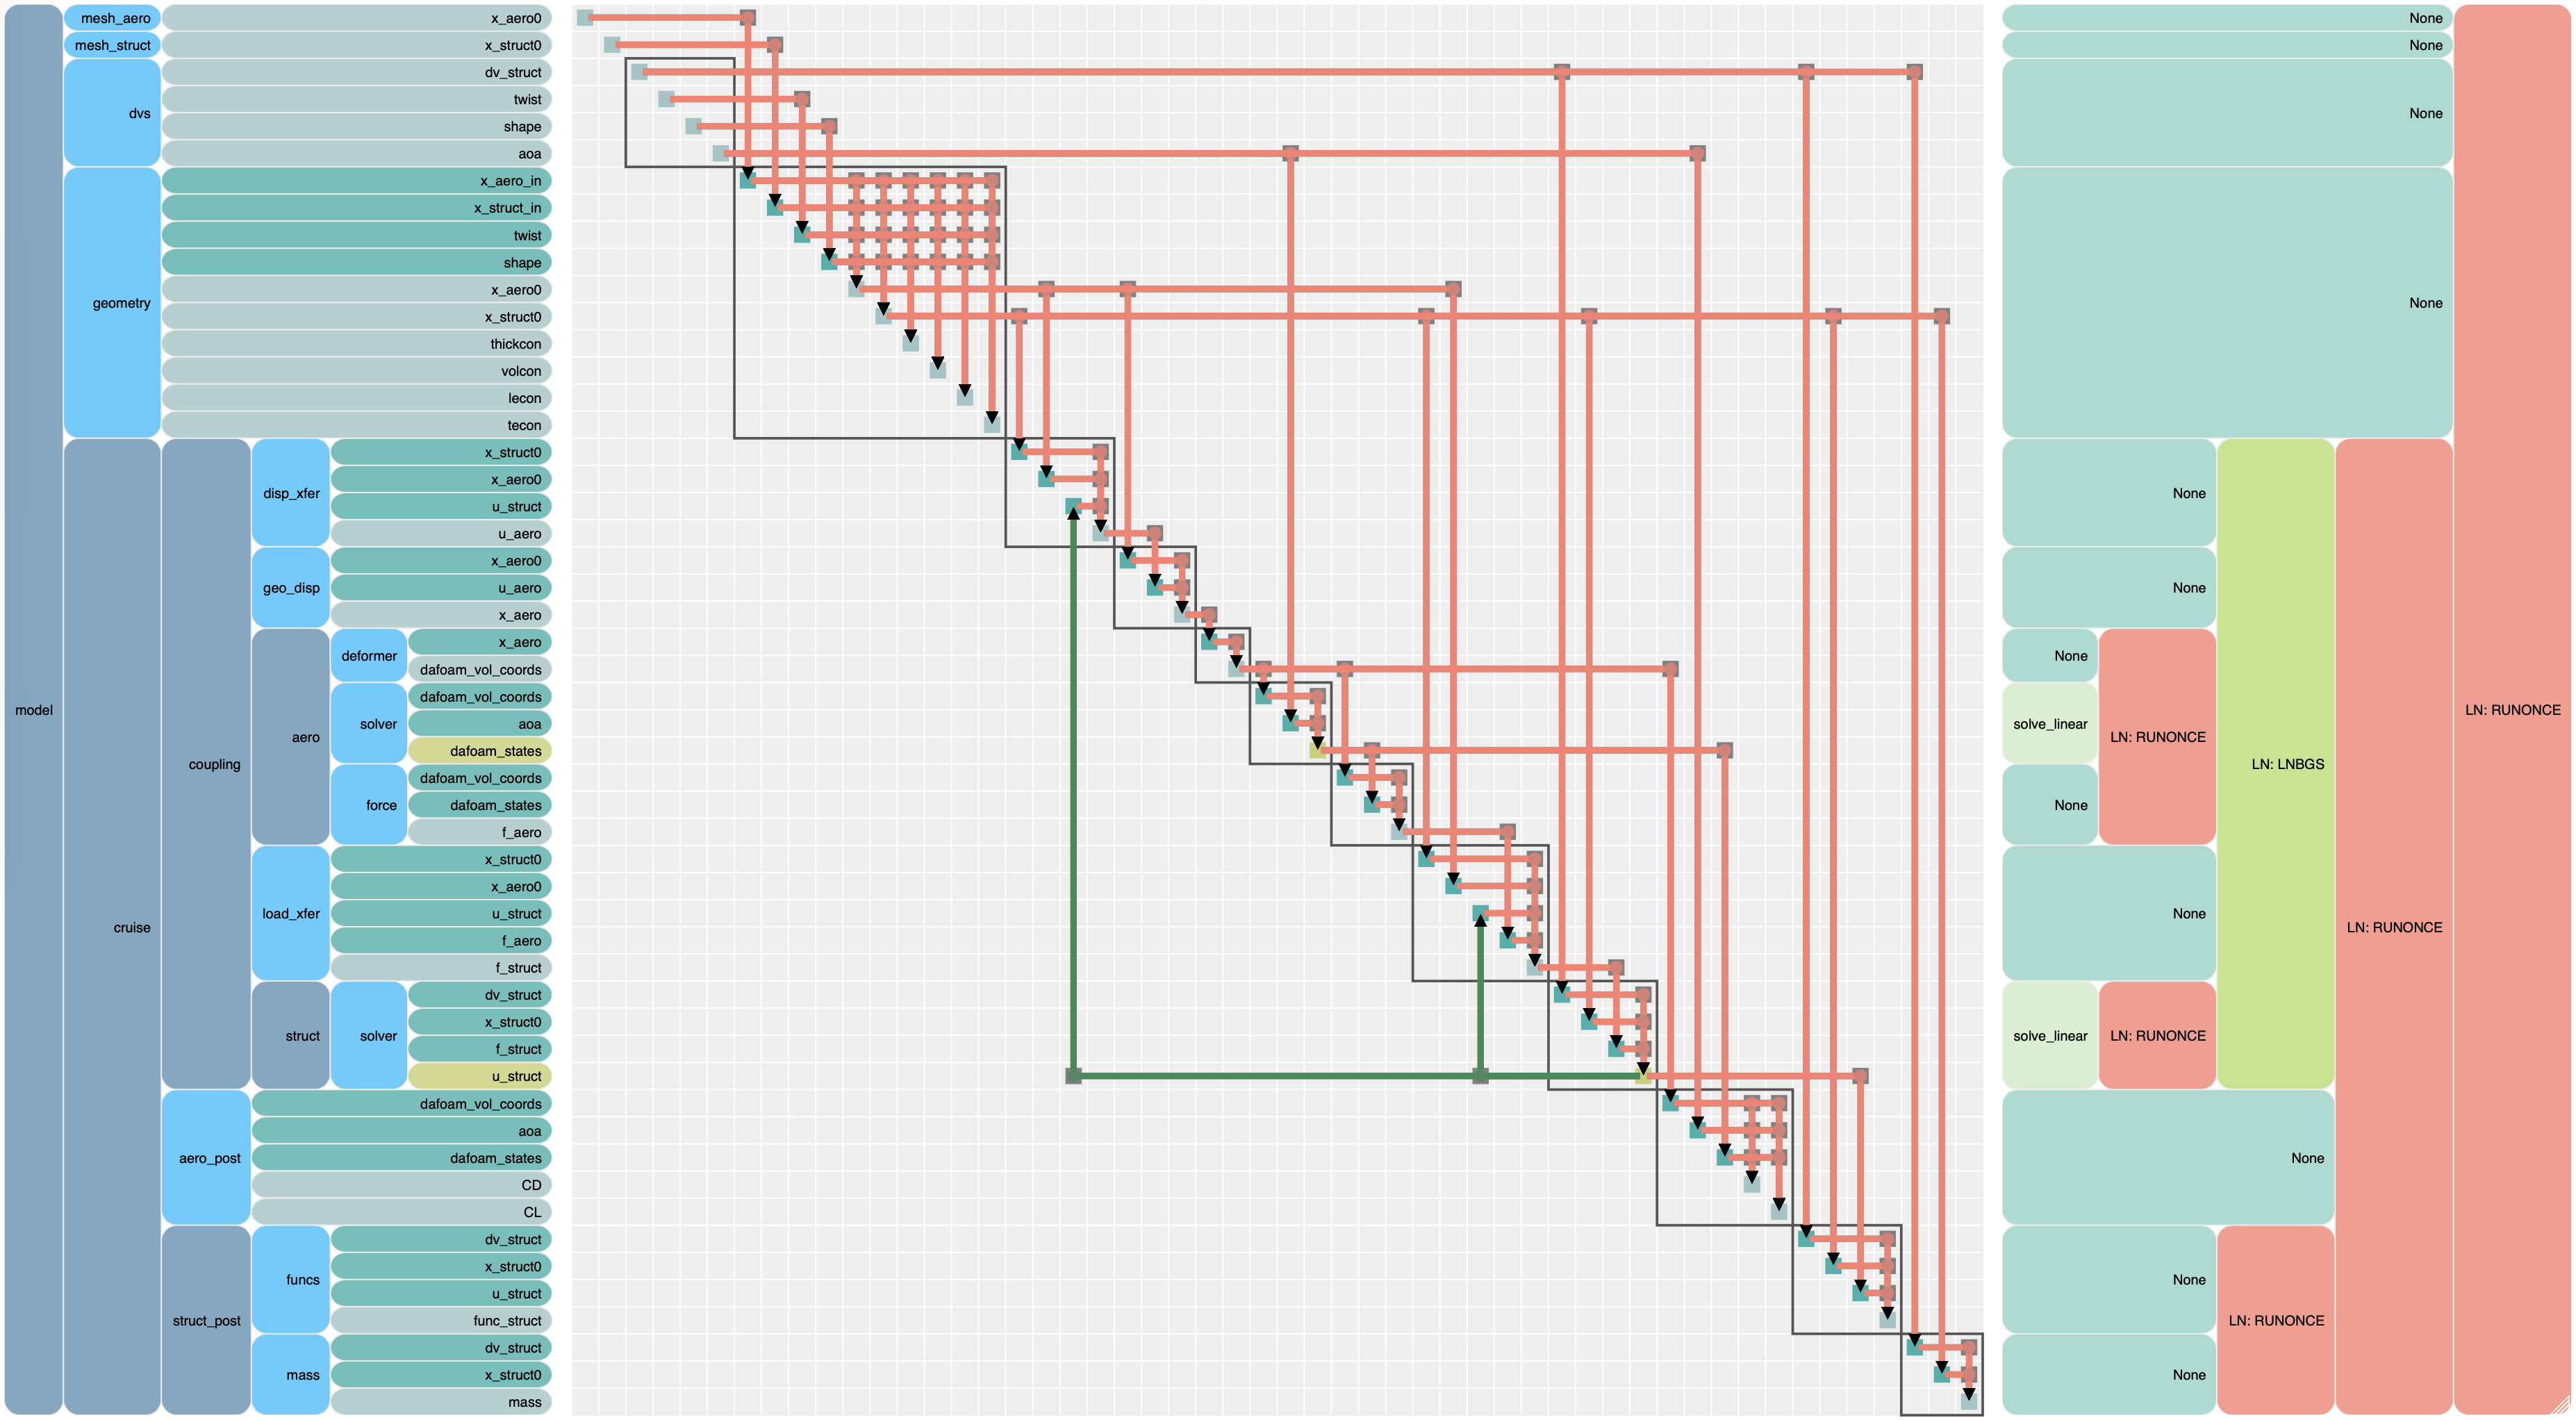
\includegraphics[width=1.0\linewidth]{images/aerostruct-n2.png}
  \caption{An N2 diagram showing aerostructural optimization. The diagram shows each component and how data is passed between them, as well as the associated solvers used for each part of the aerostructural analysis and optimization.}
  \end{figure}
\end{frame}
%---------------------------------------------------------------%

%---------------------------------------------------------------%
\begin{frame}{Analysis and Optimization Results}
  \begin{columns}
    \begin{column}{0.3\textwidth}
      \begin{center}
        Baseline
      \end{center}
    \end{column}
    \begin{column}{0.7\textwidth}
      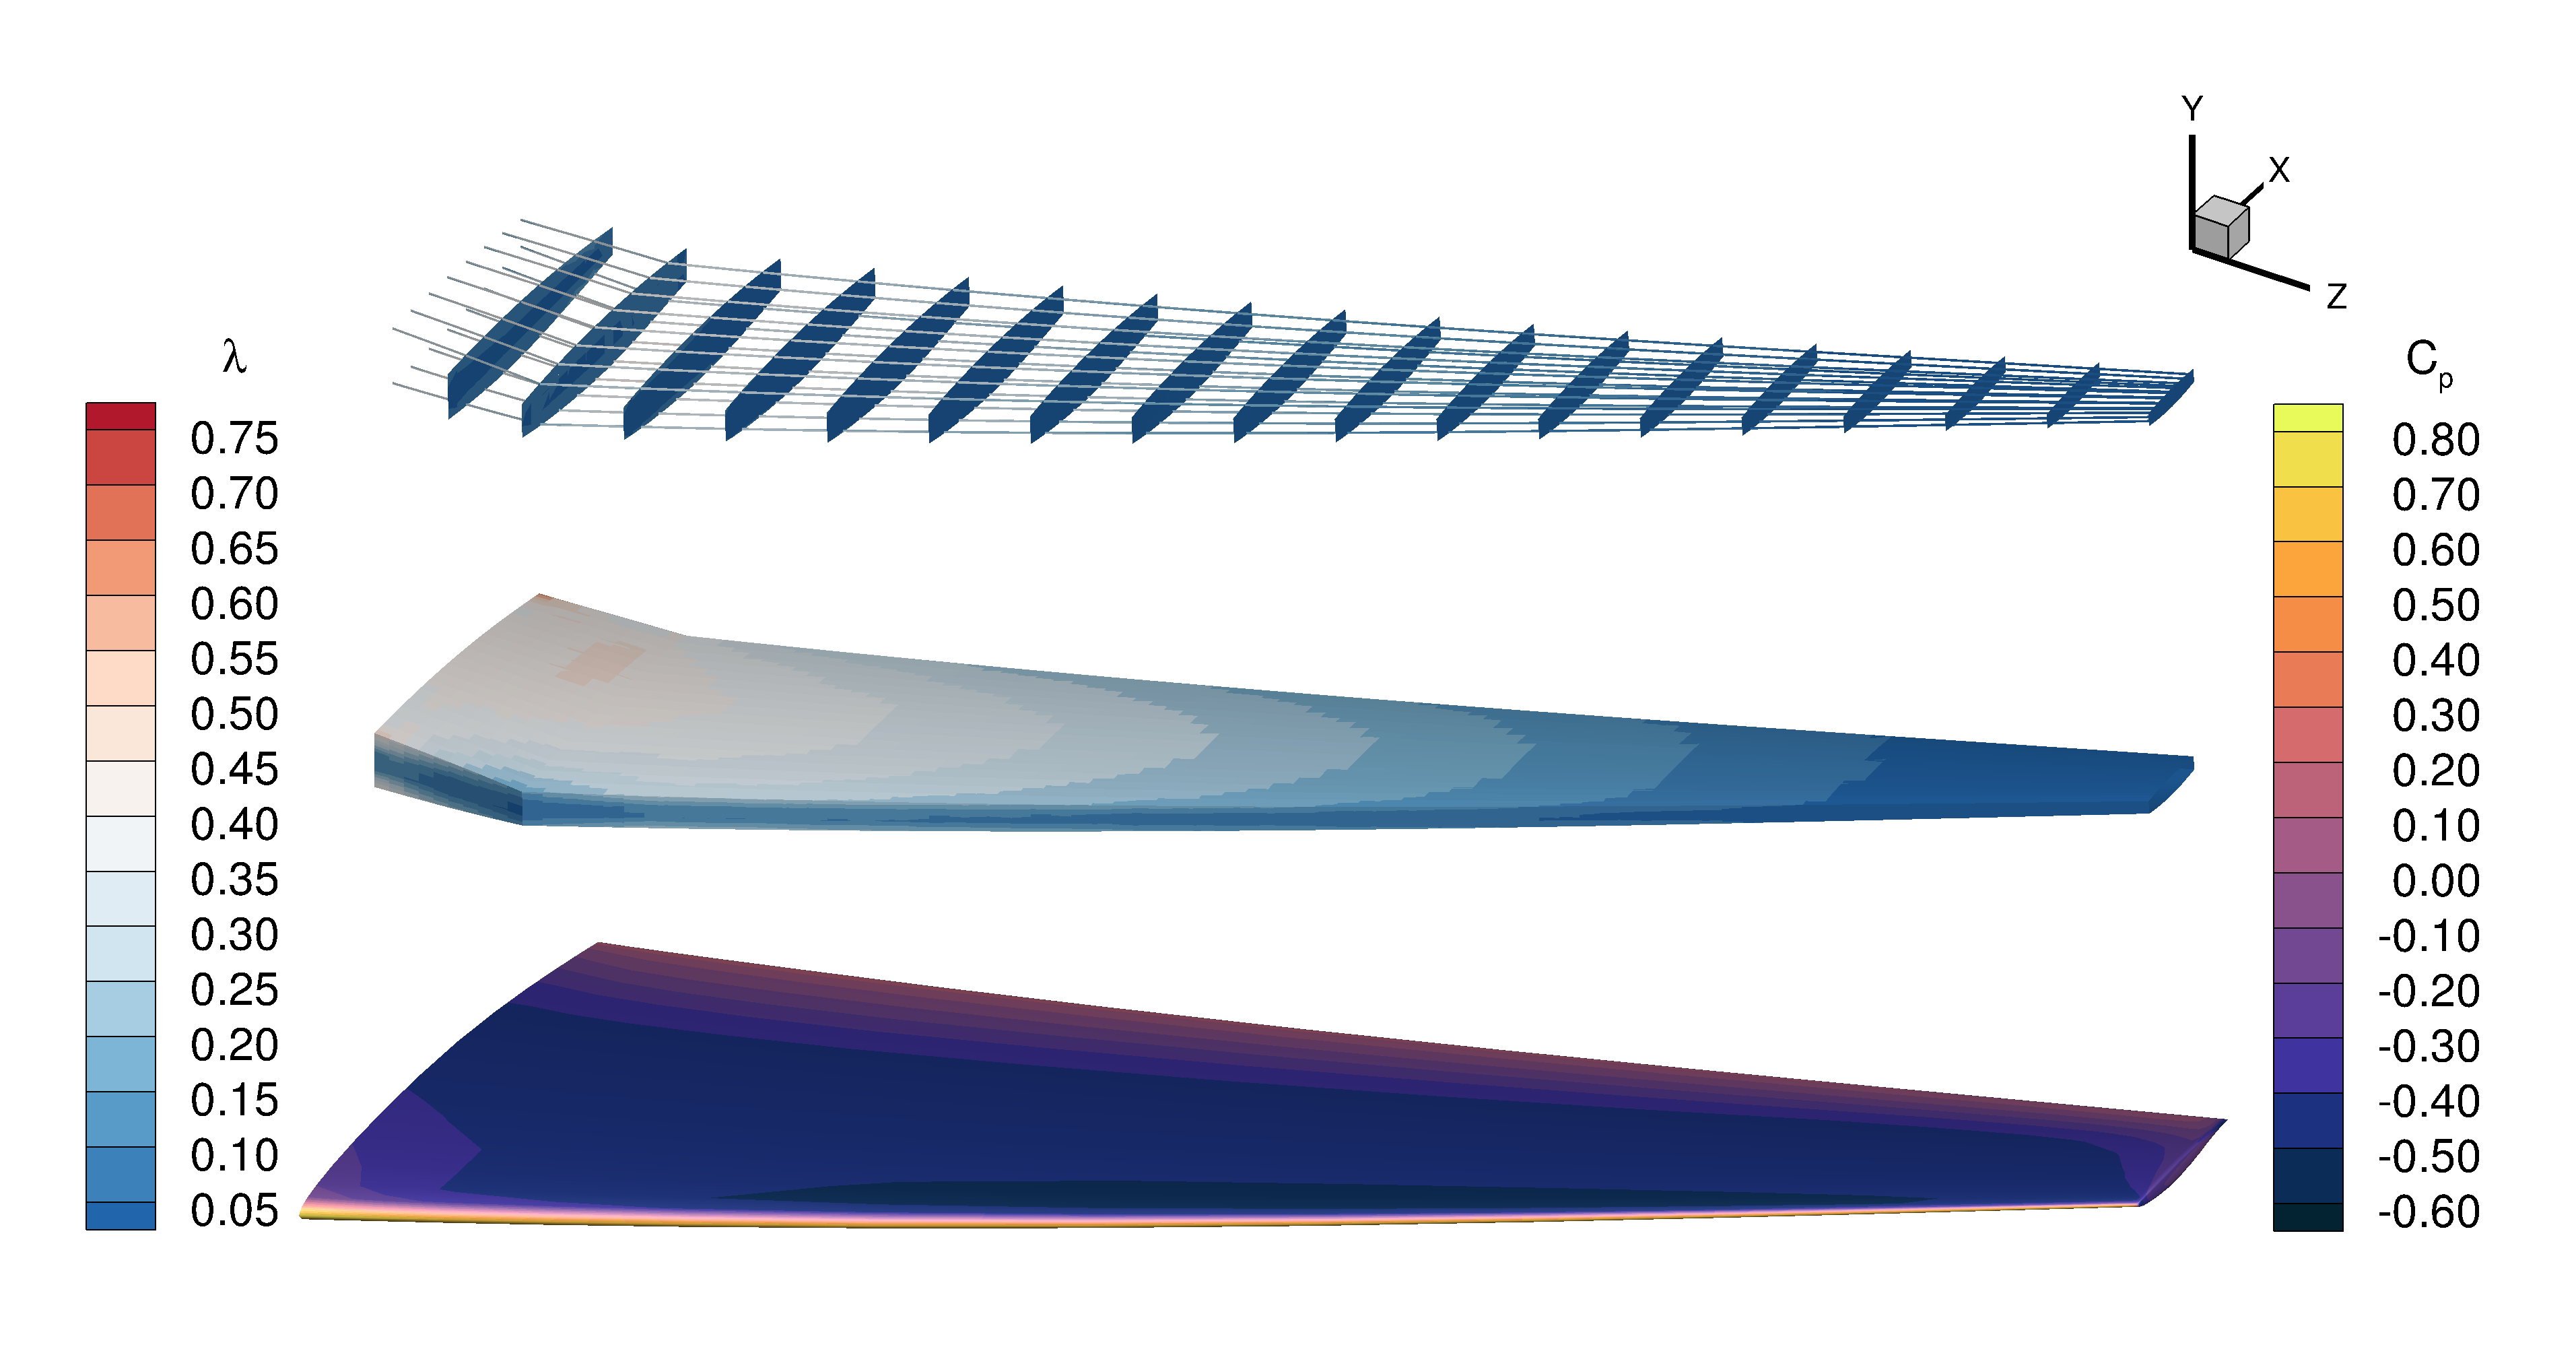
\includegraphics[width=1.0\linewidth]{images/aerostruct-resultAnalysis.png}
    \end{column}
  \end{columns}
  \noindent\rule{\textwidth}{1pt}
  \begin{columns}
    \begin{column}{0.3\textwidth}
      \begin{center}
        Optimized
      \end{center}
    \end{column}
    \begin{column}{0.7\textwidth}
      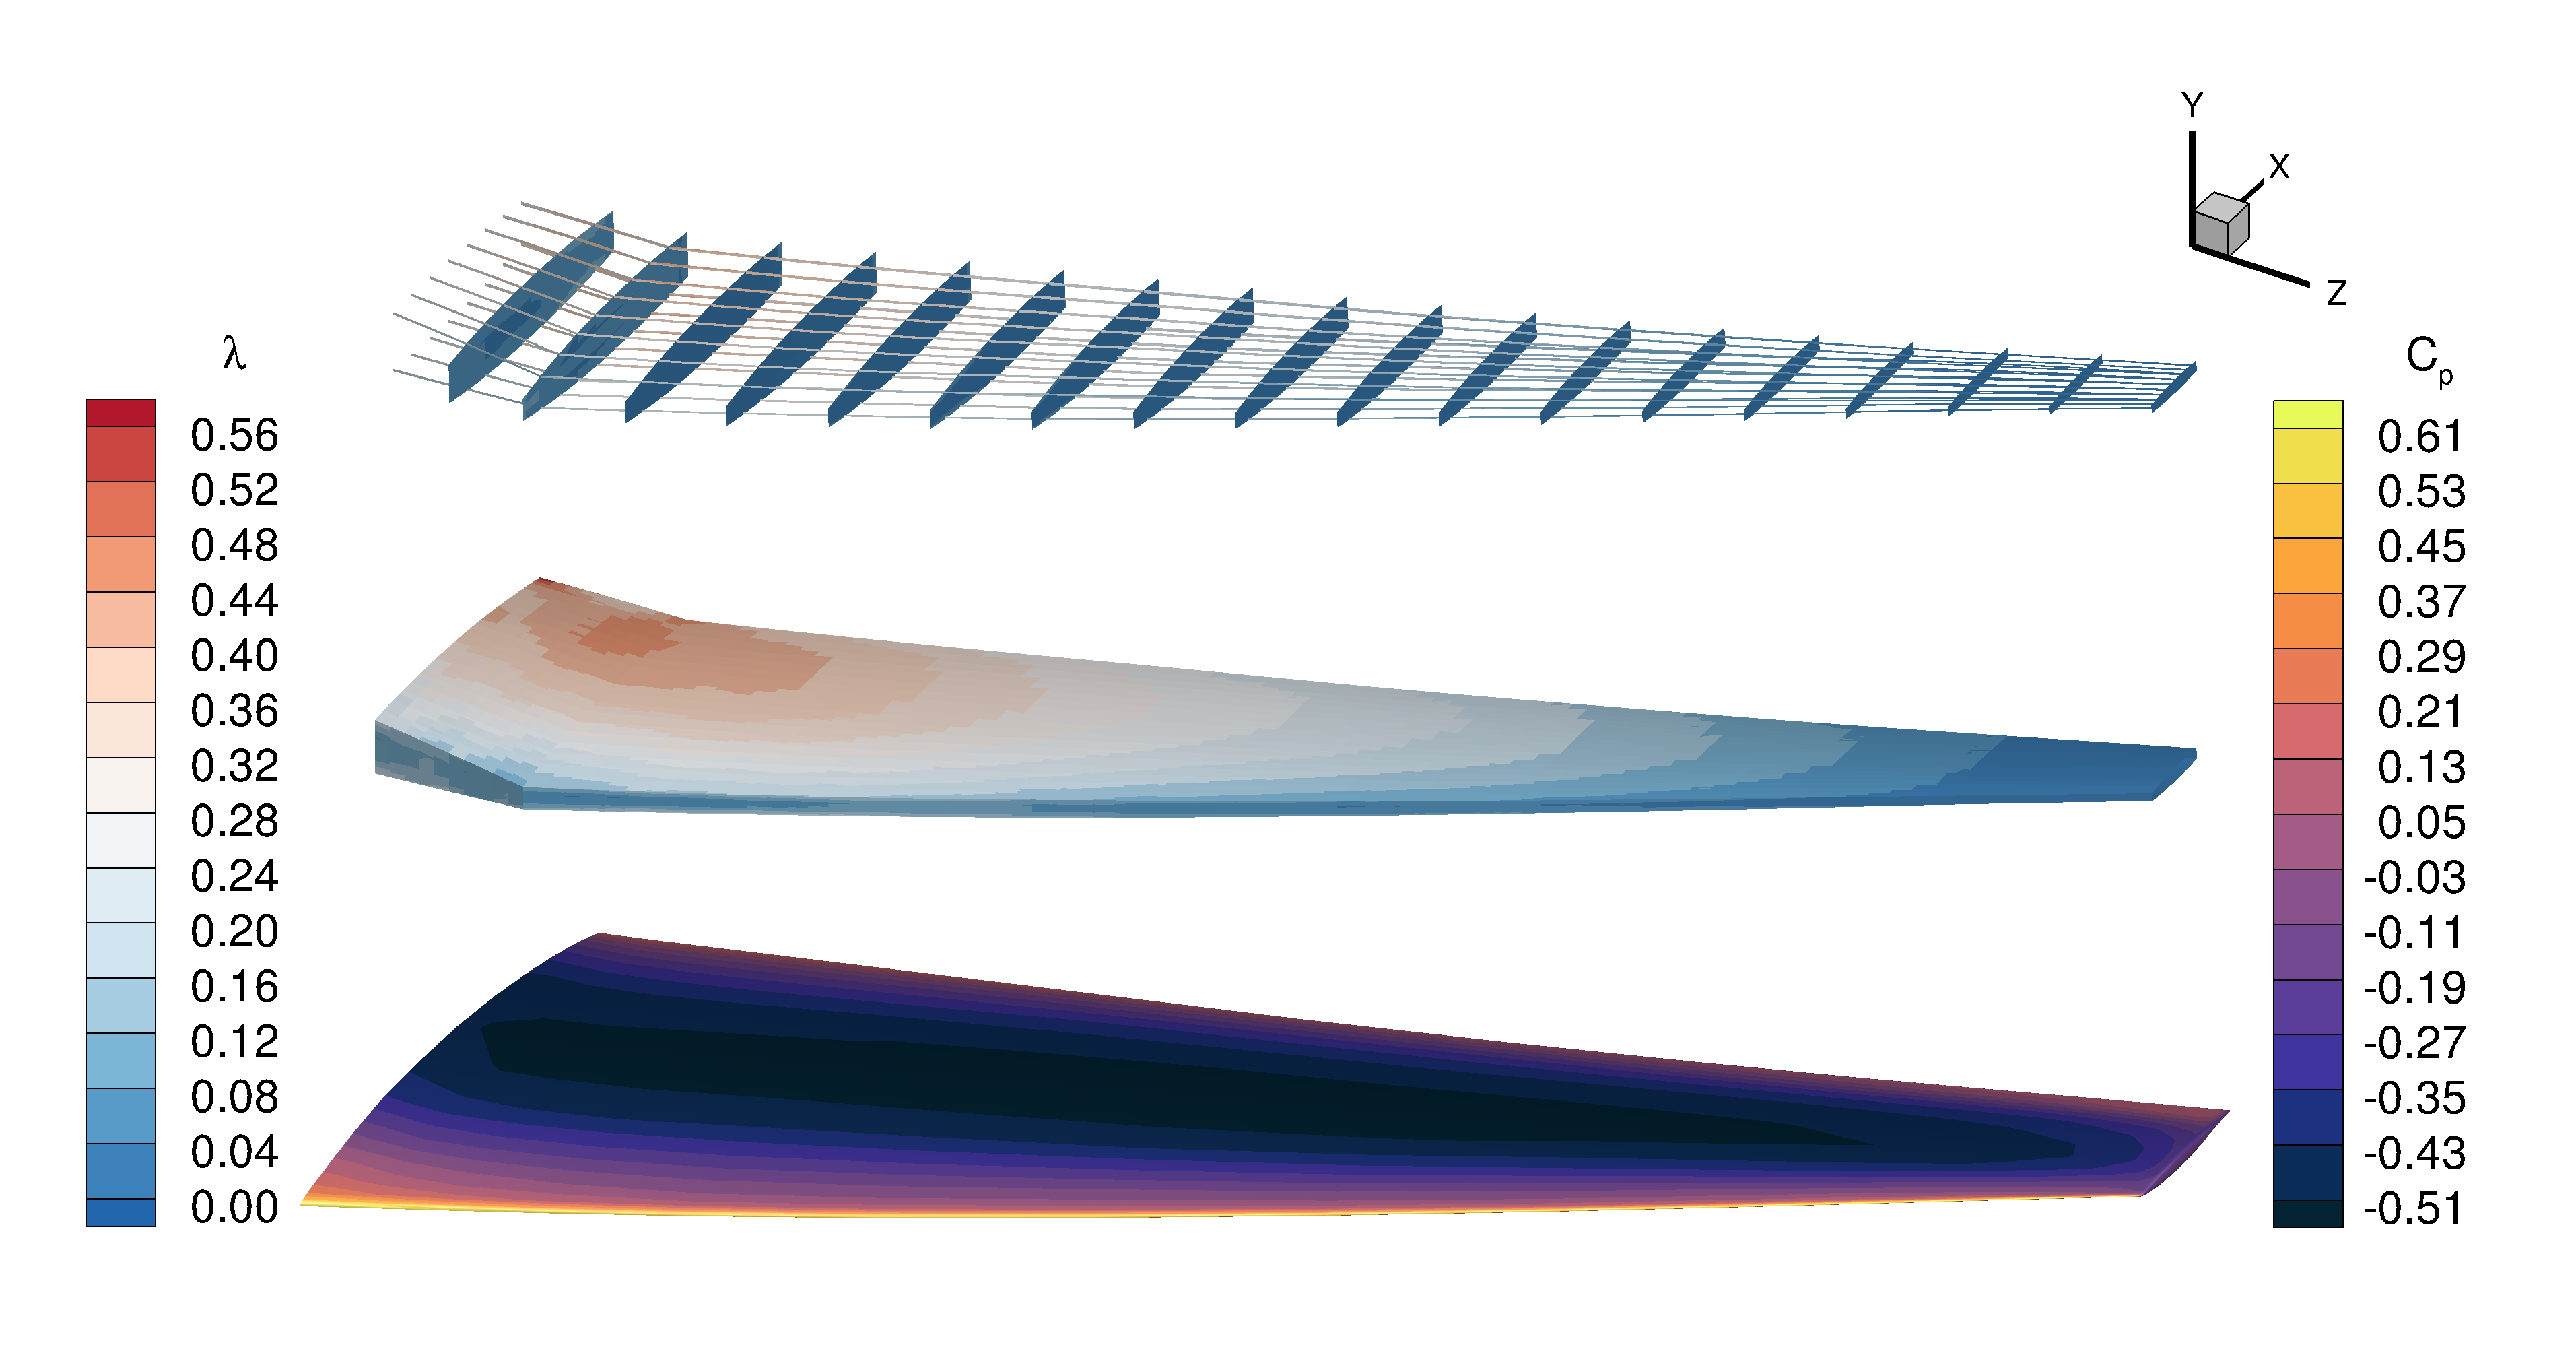
\includegraphics[width=1.0\linewidth]{images/aerostruct-resultOpt.png}
    \end{column}
  \end{columns}
\end{frame}
%---------------------------------------------------------------%

%---------------------------------------------------------------%
\begin{frame}[fragile]{Tips for Post-Processing}
  \begin{itemize}
    \setlength\itemsep{1em}
    \item Post-process the aerodynamic (DAFoam) results as for an aerodynamic case.
    \item To generate structural visualization files, use the included TACS file conversion scripts. Use "f5totec" to convert to Tecplot files or "f5tovtk" to convert to Paraview files. To generate these executables, compile them in the "extern" directory within TACS.
    \item For both Tecplot and Paraview, DAFoam will render as the deformed aerodynamic mesh of the converged aerostructural analysis / optimization. For the structural analysis, add the structural displacements to the structural mesh coordinates to visualize the deformed shape.
  \end{itemize}
\end{frame}
%---------------------------------------------------------------%

%---------------------------------------------------------------%
\begin{frame}[fragile]{Summary}
  \begin{itemize}
    \setlength\itemsep{1em}
    \item For aerostructural analysis or optimization, we couple DAFoam with TACS, a flexible, opensource, finite element solver available at \url{https://github.com/smdogroup/tacs}
    \item OpenMDAO manages the solver coupling and data passage, streamlining the configuration for the user.
    \item The runscript is largely an OpenMDAO component, defining the optimizaion scenario(s) and problem options.
  \end{itemize}
\end{frame}
%---------------------------------------------------------------%


% ************************************************************************************
\section{Add new features to DAFoam}
\renewcommand{\arraystretch}{2}

%---------------------------------------------------------------%
\begin{frame}{}
  \center \Large Add new features to DAFoam
  \normalsize
  \begin{itemize}
    \setlength\itemsep{1em}
    \item DAFoam source code structure: overview
    \item OpenFOAM layer details
    \item Cython layer details
    \item Python layer details
    \item Add a new parameter
    \item Add a new OpenFOAM layer function \& expose it to Python layer
    \item Add a new objective/constraint function
    \item Add a new model or boundary condition
    \item Add a new design variable
    \item Add a new solver
  \end{itemize}
\end{frame}
%---------------------------------------------------------------%

%---------------------------------------------------------------%
\begin{frame}{}
  \center \Large DAFoam source code structure: overview
\end{frame}
%---------------------------------------------------------------%

%---------------------------------------------------------------%
\begin{frame}{Three code layers: OpenFOAM, Cython, and Python}
\begin{figure}
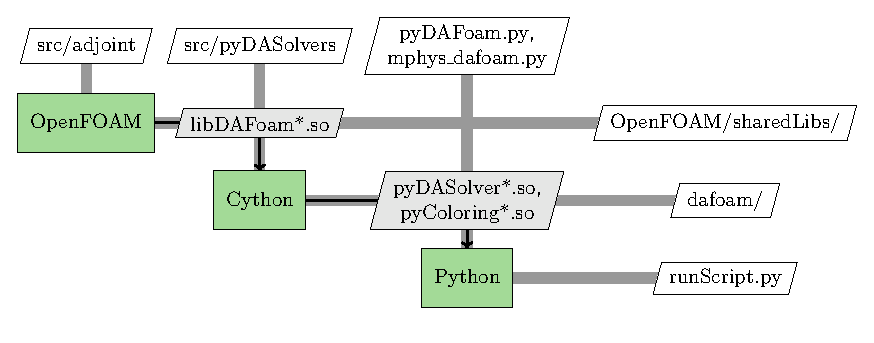
\includegraphics[width=1.05\linewidth]{images/dafoam_layers.pdf} 
\caption{There are three code layers in DAFoam: OpenFOAM, Cython, and Python. Each layer takes source code or libraries as the input in the vertical direction and output libraries to the horizontal direction.}
\end{figure}
\end{frame}
%---------------------------------------------------------------%


%---------------------------------------------------------------%
\begin{frame}[fragile]{OpenFOAM layer overview}
  The OpenFOAM layer contains C++ classes for the OpenFOAM primal solvers and the discrete adjoint classes to compute derivatives. The OpenFOAM layer's source codes are in dafoam/src/adjoint.
  \begin{itemize}
    \setlength\itemsep{1em}
    \item When DAFoam is compiled with the original mode, it will generate dynamic libraries for three different conditions: incompressible, compressible, and solid. In other words, it will compile three libDAFoam*.so files. Refer to dafoam/src/adjoint/Make/files\_Incompressible for which files are compiled for the incompressible case
    \item When DAFoam is compiled with the ADR (reverse-mode AD) or ADF (forward-mode AD) modes, it will generate six more libDAFoam*.so libraries.
    \item These libraries will be saved to dafoam/OpenFOAM/sharedLibs
    \item To avoid file IO during optimization, we rewrite all the OpenFOAM solvers (binary executives) as libraries such that we can call them from Python
  \end{itemize}
\end{frame}
%---------------------------------------------------------------%

%---------------------------------------------------------------%
\begin{frame}[fragile]{Cython layer overview}
The compiled libDAFoam*.so from the OpenFOAM layer are pure C++ libraries, so they cannot be directly called from Python. We need to wrap these libraries using Cython. The Cython layer source codes are in src/pyDASolvers
  \begin{itemize}
    \setlength\itemsep{1em}
    \item The Cython layer solver will use the libDAFoam*.so libraries from the OpenFOAM layer
    \item When running the \texttt{Allmake} command, both OpenFOAM and Cython libraries will be compiled
    \item Similar to the OpenFOAM layer, we will compile three sets of Cython libraries for both pyDASolver*.so and pyColoringSolver*.so. These libraries will be saved to dafoam/dafoam folder.
    \item pyDASolver*.so and pyColoringSolver*.so are the Cython libraries callable from the Python layer
    
  \end{itemize}
\end{frame}
%---------------------------------------------------------------%

%---------------------------------------------------------------%
\begin{frame}[fragile]{Python layer overview}
When running \texttt{pip install .}, all the files (pyDASolver*.so, pyDAFoam.py, mphys\_dafoam.py, etc.) in the dafoam/dafoam folder will be copied to miniconda3/lib/python3.8/site-packages/dafoam, and they become importable from runScript.py

\begin{itemize}
  \setlength\itemsep{1em}
    \item runScript.py interacts with the Python layer only, it can not directly access the OpenFOAM or Cython libraries.
    \item The Python layer's main entry point is the \texttt{DAFoamBuilder} class from mphys\_dafoam.py. So in runScript.py we import DAFoamBuilder. DAFoamBuilder then call other Python interfaces from pyDAFoam.py
    \item pyDAFoam.py actually imports pyDASolvers*.so (solve primal and adjoint) and pyColoringSolver*.so (calculate coloring) in its \texttt{\_\_initSolver()} function
    \item Other moudles (e.g., pyGeo, IDWarp) have their own Python interfaces written in Mphys, so runScript.py imports them too  
  \end{itemize}
\end{frame}
%---------------------------------------------------------------%

%---------------------------------------------------------------%
\begin{frame}{}
  \center \Large OpenFOAM layer details
\end{frame}
%---------------------------------------------------------------%

%---------------------------------------------------------------%
\begin{frame}[fragile]{Folder structure in dafoam/src/adjoint}
The source codes for the OpenFOAM layer are in src/adjoint. Each subfolder defines a class.
\footnotesize
\lstset{ language=bash }
\begin{lstlisting}
src/adjoint
  Allclean           DAIndex            DAOption           DAUtility
  Allmake            DAJacCon           DAPartDeriv        Make
  DACheckMesh        DALinearEqn        DARegDb            boundaryConditions
  DAColoring         DAModel            DAResidual         lnInclude
  DAField            DAMotion           DASolver           models
  DAFvSource         DAObjFunc          DAStateInfo
\end{lstlisting}
\normalsize

If a class has no child classes, it reads
\footnotesize
\lstset{ language=bash }
\begin{lstlisting}
src/adjoint/DAIndex
  DAIndex.C DAIndex.H
\end{lstlisting}
\normalsize

Otherwise, it reads.
\footnotesize
\lstset{ language=bash }
\begin{lstlisting}
src/adjoint/DAObjFunc
  DAObjFunc.C       DAObjFuncForce.C    DAObjFuncMoment.C
  DAObjFunc.H       DAObjFuncForce.H    DAObjFuncMoment.H
  ...........       ................    .................
\end{lstlisting}
\normalsize

Here DAObjFuncForce is one of the child classes for DAObjFunc.

\end{frame}
%---------------------------------------------------------------%

%---------------------------------------------------------------%
\begin{frame}[fragile]{OpenFOAM layer's main entry point: DASolver class}
The DASolver class is the main interface for the OpenFOAM layer.
\footnotesize
\lstset{ language=bash }
\begin{lstlisting}
src/adjoint/DASolver
  DALaplacianFoam         DARhoSimpleFoam             DASolver.C
  DAPimpleDyMFoam         DAScalarTransportFoam       DASolver.H
  DAPimpleFoam            DASimpleFoam                DATurboFoam
  DAPisoFoam              DASimpleTFoam
  DARhoSimpleCFoam        DASolidDisplacementFoam
\end{lstlisting}
\normalsize

In DASolver.H, we define primal and adjoint functions to interface with the Python layer, e.g., initSolver, solvePrimal, calcdRdWT, solveLinearEqn. The adjoint functions are universal to all solvers. solvePrimal() is a virtual function that needs to be defined by each child class/solver. 

For example, the child class DASimpleFoam defines its own solvePrimal function that follows the exact same solution process as OpenFOAM's original simpleFoam solver.

\footnotesize
\lstset{ language=bash }
\begin{lstlisting}
src/adjoint/DASolver/DASimpleFoam
  DASimpleFoam.C       UEqnSimple.H         createRefsSimple.H
  DASimpleFoam.H       createFieldsSimple.H pEqnSimple.H
\end{lstlisting}
\normalsize
\end{frame}
%---------------------------------------------------------------%

%---------------------------------------------------------------%
\begin{frame}[fragile]{DASolver$-$DASimpleFoam example (1/4)}
\texttt{initSolver()} and \texttt{solvePrimal()} are the main virtual functions implemented in DASimpleFoam.C.
\footnotesize
\lstset{ language=c++ }
\begin{lstlisting}
void DASimpleFoam::initSolver(){
  Info << "Initializing fields for DASimpleFoam" << endl;
  // get the reference for runTime and mesh objects these two variables 
  // have been initialized in DASolver constructor: DASolver.C line 48
  Time& runTime = runTimePtr_();
  fvMesh& mesh = meshPtr_();
  // initialize field variables
  #include "createSimpleControlPython.H"
  #include "createFieldsSimple.H"
  // initialize the adjoint classes, e.g., DAIndex, DAOption, DATurbo
  // NOTE: this file is in dafoam/src/adjoiont/include
  #include "createAdjointIncompressible.H"
  // initialize checkMesh object
  daCheckMeshPtr_.reset(new DACheckMesh(daOptionPtr_(), runTime, mesh));
  // initialize adjoint linear equation solution object
  daLinearEqnPtr_.reset(new DALinearEqn(mesh, daOptionPtr_()));
  // initialize the objective function
  this->setDAObjFuncList();

  .... }
\end{lstlisting}
\normalsize

\end{frame}
%---------------------------------------------------------------%

%---------------------------------------------------------------%
\begin{frame}[fragile]{DASolver$-$DASimpleFoam example (2/4)}
  \texttt{solvePrimal()} uses xvVec (volume coordinates) as the input and calculates wVec (state variables). xvVec and wVec are Petsc vectors.
\footnotesize
\lstset{ language=c++ }
\begin{lstlisting}
void DASimpleFoam::solvePrimal(const Vec xvVec, Vec wVec){
  // create the references for the pointer objects
  #include "createRefsSimple.H"
  #include "createFvOptions.H"
  // change the run status, this is needed for the fvSource object
  daOptionPtr_->setOption<word>("runStatus", "solvePrimal");
  // call correctNut, this is equivalent to turbulence->validate();
  daTurbulenceModelPtr_->updateIntermediateVariables();
  Info << "\nStarting time loop\n" << endl;
  // deform the mesh based on the xvVec, we essentially assign the values 
  // in xvVec to the OpenFOAM's mesh coordinates
  this->pointVec2OFMesh(xvVec);
  // check mesh quality, if the mesh quality fails, do not run the primal
  label meshOK = this->checkMesh();
  if (!meshOK)
  {
    this->writeFailedMesh();
    return 1;
  }
  .... }
\end{lstlisting}
\normalsize

\end{frame}
%---------------------------------------------------------------%

%---------------------------------------------------------------%
\begin{frame}[fragile]{DASolver$-$DASimpleFoam example (3/4)}
The main loop, which is same as the origional simpleFoam solver
\footnotesize
\lstset{ language=c++ }
\begin{lstlisting}
  while (this->loop(runTime))
  {
      printToScreen = this->isPrintTime(runTime, printInterval);
      if (printToScreen){
          Info << "Time = " << runTime.timeName() << nl << endl;}
      p.storePrevIter();
      // --- Pressure-velocity SIMPLE corrector
      #include "UEqnSimple.H"
      #include "pEqnSimple.H"
      laminarTransport.correct();
      daTurbulenceModelPtr_->correct();
      // we print the residual to screen every 100 steps
      if (printToScreen)
      {
          daTurbulenceModelPtr_->printYPlus();
          this->printAllObjFuncs();
          Info << "ExecutionTime = " << runTime.elapsedCpuTime() << " s"
               << "  ClockTime = " << runTime.elapsedClockTime() << " s" << nl << endl;
      }
      runTime.write();
  }
\end{lstlisting}
\normalsize

\end{frame}
%---------------------------------------------------------------%


%---------------------------------------------------------------%
\begin{frame}[fragile]{DASolver$-$DASimpleFoam example (4/4)}

After the simulation is done, we need to do the following
\footnotesize
\lstset{ language=c++ }
\begin{lstlisting}

  // write the intermediate fields
  this->writeAssociatedFields();
  // calculate the converged primal residual norm
  this->calcPrimalResidualStatistics("print");
  // primal converged, assign the OpenFoam fields to the state vec wVec
  this->ofField2StateVec(wVec);
  // write the deformed mesh to files
  mesh.write();
  Info << "End\n"<< endl;

  // check if the primal residual drops to the prescribed tolerance
  // if not, return failed for this primal run
  return this->checkResidualTol();
\end{lstlisting}
\normalsize

\end{frame}
%---------------------------------------------------------------%

%---------------------------------------------------------------%
\begin{frame}[fragile]{Adjoint functions in DASolver}

Essentially, any adjoint functions we want to call in the Python layer need to be defined in DASolver.C and DASolver.H. Here are just a few examples.
\footnotesize
\lstset{ language=c++ }
\begin{lstlisting}
// function to compute dF/dW for the adjoint equation rhs
void DASolver::calcdFdWAD(
  const Vec xvVec,
  const Vec wVec,
  const word objFuncName,
  Vec dFdW)
{
  .....
}

// function to extract force from the wing surface for aerostructural
void DASolver::getForces(Vec fX, Vec fY, Vec fZ, Vec pointList)
{
  .....
}

// return the objective function value givne the function name
scalar DASolver::getObjFuncValue(const word objFuncName)
{
  ......
}
\end{lstlisting}
\normalsize

\end{frame}
%---------------------------------------------------------------%

%---------------------------------------------------------------%
\begin{frame}[fragile]{Original, reverse- and forward-AD OpenFOAM codes}

\begin{itemize}
  \setlength\itemsep{0.5em}
\item To faciliate the optimization, we have used an operator-overloading automatic differentiation (AD) tool called CoDiPack (\url{https://github.com/SciCompKL/CoDiPack}) to differentiate the OpenFOAM's source code. The AD version of OpenFOAM is avaiable at \url{https://github.com/DAFoam/OpenFOAM-v1812-AD}

\item When differentiated, the OpenFOAM calculation becomes $\sim$3 times slower than the original version. Therefore, we use the AD version for the adjoint but not for running the primal.

\item To enable this, we have compiled OpenFOAM into three versions: original, ADR (reverse AD), and ADF (forward AD).

\item The forward- and reverse-AD versions of OpenFOAM libraries have names end with ADR and ADF. For example, we will have finiteVolume.so, finiteVolumeADR.so, and finiteVolumeADF.so. With this treatment, we can allow loading both original and ADR libraries during the optimization in the Python layer.

\end{itemize}


\end{frame}
%---------------------------------------------------------------%


%---------------------------------------------------------------%
\begin{frame}{}
  \center \Large Cython layer details
\end{frame}
%---------------------------------------------------------------%


%---------------------------------------------------------------%
\begin{frame}[fragile]{Folder structure in dafoam/src/pyDASolvers}
As mentioned above, to wrap the C++ libraries from the OpenFOAM layer, we define a C++ class called DASolvers (DASolvers.H and DASolvers.C), and its corresponding Cython class is called pyDASolvers (pyDASolver.pyx).
\footnotesize
\lstset{ language=bash }
\begin{lstlisting}
src/pyDASolvers
  Allclean                DASolvers.H             setup_Incompressible.py
  Allmake                 pyDASolvers.pyx         setup_Solid.py
  DASolvers.C             setup_Compressible.py
\end{lstlisting}
\normalsize

A few notes:

\begin{itemize}
  \setlength\itemsep{0.5em}
 \item DASolver (OpenFOAM layer) and DASolvers (Cython layer) are two different C++ classes.
 \item We do not directly wrap the DASolver class with Cython, instead, we create the DASolvers class to call the DASolver class. This treatment allows DASolver to become a pure C++ library that can easily use the runtime selction mechanism (e.g., child class for turbulence models) in OpenFOAM.
 \item The DASolvers and pyDASolvers are pure wrapper classes so they do not handle child classes or virtual functions
\end{itemize}

\end{frame}
%---------------------------------------------------------------%

%---------------------------------------------------------------%
\begin{frame}[fragile]{DASolvers class}
 As mentioned above, what DASolvers class does is to call the DASolver's methods implemented in the OpenFOAM layer. So DASolvers.H will receive the DASolver object and call DASolver's methods
\footnotesize
\lstset{ language=c++ }
\begin{lstlisting}
class DASolvers
{
  // DASolverPtr_ is initialized in DASolvers.C
  // initialize fields and variables
  void initSolver()
  {
      // call DASolverPtr's initSolver method
      DASolverPtr_->initSolver();
  }
  // solve the primal equations
  label solvePrimal(
      const Vec xvVec,
      Vec wVec)
  {
      // call DASolverPtr's solvePrimal method
      return DASolverPtr_->solvePrimal(xvVec, wVec);
  }
}
\end{lstlisting}
\normalsize
\end{frame}
%---------------------------------------------------------------%

%---------------------------------------------------------------%
\begin{frame}[fragile]{pyDASolvers class}
pyDASolvers is written in Cython format. We need to wrap all the DASolvers' member and expose them to the Python layer. To to so, we need to first define them in \texttt{cppclass DASolvers:}. Then, we need to define them in \texttt{cdef class pyDASolvers:}. 

See the following for how initSolver and solverPrimal are wrapped.

\footnotesize
\lstset{ language=python }
\begin{lstlisting}
# declare cpp functions
cdef extern from "DASolvers.H" namespace "Foam":
    cppclass DASolvers:
        DASolvers(char *, object) except +
        void initSolver()
        int solvePrimal(PetscVec, PetscVec)

# create python wrappers that call cpp functions
cdef class pyDASolvers:
    # wrap all the other member functions in the cpp class
    def initSolver(self):
        self._thisptr.initSolver()

    def solvePrimal(self, Vec xvVec, Vec wVec):
        return self._thisptr.solvePrimal(xvVec.vec, wVec.vec)
\end{lstlisting}
\normalsize
\end{frame}
%---------------------------------------------------------------%

%---------------------------------------------------------------%
\begin{frame}[fragile]{A few notes about the Cython layer}


\begin{itemize}
  \setlength\itemsep{0.5em}
 \item We can not directly pass a Python array to the OpenFOAM layer. We have to pass them as Petsc Vector or Matrix.
 \item When passing a char type variable to the OpenFOAM layer, we need to need to use var\_name.encode() in the Python layer.
 \item The Python layer can call OpenFOAM layer's member; however, the OpenFOAM layer can not call Python layer's members.
\end{itemize}
  
\end{frame}
%---------------------------------------------------------------%



%---------------------------------------------------------------%
\begin{frame}{}
  \center \Large Python layer details
\end{frame}
%---------------------------------------------------------------%


%---------------------------------------------------------------%
\begin{frame}[fragile]{Folder structure in dafoam}
The Python layer codes are in the dafoam folder, see below. You may also see a few *.so libraries after compiling DAFoam. The two main Python layer files are pyDAFoam.py and mphys\_dafoam.py
\footnotesize
\lstset{ language=bash }
\begin{lstlisting}
dafoam
  __init__.py    mphys/mphys_dafoam.py     optFuncs.py    
  pyDAFoam.py    scripts
\end{lstlisting}
\normalsize

The scripts folder contains some useful utility python functions, e.g., to convert the plot3d to tecplot format, to transform or rotate a stl file.
\end{frame}
%---------------------------------------------------------------%


%---------------------------------------------------------------%
\begin{frame}[fragile]{pyDAFoam.py overview: PYDAFOAM}
PYDAFOAM is the main entry point to pyDAFoam.py, and it will call initSolver() method from the OpenFOAM layer to initialize variables for both primal and adjoint solvers.
\footnotesize
\lstset{ language=python }
\begin{lstlisting}
class PYDAFOAM(object):
  def __init__(self, comm=None, options=None):
      """
      Initialize class members
      """
      self.version = __version__
      # name
      self.name = "PYDAFOAM"
      # initialize options for adjoints
      self._initializeOptions(options)
      # check if the combination of options is valid.
      self._checkOptions()
      # initialize comm for parallel communication
      self._initializeComm(comm)
      ......
      # register solver names and set their types
      self._solverRegistry()
      # initialize the pySolvers
      self.solverInitialized = 0
      self._initSolver()
\end{lstlisting}
\normalsize

\end{frame}
%---------------------------------------------------------------%


%---------------------------------------------------------------%
\begin{frame}[fragile]{pyDAFoam.py overview: DAOPTION}
The DAOPTION class in pyDAFoam.py defines the parameters for DAFoam optimization and assign inital values to them.
\footnotesize
\lstset{ language=python }
\begin{lstlisting}
class DAOPTION(object):
  def __init__(self, comm=None, options=None):
      self.solverName = "DASimpleFoam"
      self.primalMinResTol = 1.0e-8
      self.primalBC = {}
\end{lstlisting}
\normalsize

Then it will be used by the PYDAFOAM class from:

\footnotesize
\lstset{ language=python }
\begin{lstlisting}
def _getDefOptions(self):
    # initialize the DAOPTION object
    daOption = DAOPTION()
    defOpts = {}
    # assign all the attribute of daOptoin to defOpts
    for key in vars(daOption):
        value = getattr(daOption, key)
        defOpts[key] = [type(value), value]
    return defOpts
\end{lstlisting}
\normalsize

Note that the above \texttt{getDefOptions} will be called by \texttt{initializeOptions} from the PYDAFOAM's \texttt{init()} function

\end{frame}
%---------------------------------------------------------------%

%---------------------------------------------------------------%
\begin{frame}[fragile]{mphys\_dafoam.py overview: DAFoamBuilder}
The DAFoamBuilder is the main entry point for mphys\_dafoam.py. It will call PYDAFOAM class from pyDAFoam.py to initialize OpenFOAM layer variables, and also return a DAFoamGroup (see next slide)
\footnotesize
\lstset{ language=python }
\begin{lstlisting}
class DAFoamBuilder(Builder):
  # api level method for all builders
  def initialize(self, comm):
      # initialize the PYDAFOAM class, defined in pyDAFoam.py
      self.DASolver = PYDAFOAM(options=self.options, comm=comm)
      # always set the mesh
      mesh = USMesh(options=self.mesh_options, comm=comm)
      self.DASolver.setMesh(mesh)
  # api level method for all builders
  def get_coupling_group_subsystem(self, scenario_name=None):
      dafoam_group = DAFoamGroup(
          solver=self.DASolver,
          use_warper=self.warp_in_solver,
          struct_coupling=self.struct_coupling,
          prop_coupling=self.prop_coupling,
      )
      return dafoam_group
\end{lstlisting}
\normalsize

\end{frame}
%---------------------------------------------------------------%

%---------------------------------------------------------------%
\begin{frame}[fragile]{mphys\_dafoam.py overview: DAFoamGroup}
The DAFoamGroup will add relevant component for analysis and optimization. It will also add the DAFoamSolver component (see next slide).
\footnotesize
\lstset{ language=python }
\begin{lstlisting}
class DAFoamGroup(Group):
  def setup(self):
      # add the IDWarp component for mesh deformation
      if self.use_warper:
          self.add_subsystem(
              "deformer",
              DAFoamWarper(solver=self.DASolver),
              promotes_inputs=["x_aero"],
              promotes_outputs=["dafoam_vol_coords"],
          )
      # add the solver implicit component from DAFoamSolver
      self.add_subsystem(
          "solver",
          DAFoamSolver(solver=self.DASolver, prop_coupling=self.prop_coupling),
          promotes_inputs=["*"],
          promotes_outputs=["dafoam_states"],
      )

\end{lstlisting}
\normalsize

\end{frame}
%---------------------------------------------------------------%


%---------------------------------------------------------------%
\begin{frame}[fragile]{mphys\_dafoam.py overview: DAFoamSolver}
The DAFoamSolver implements the way to compute the adjoint matrix-vector product using AD and solve the adjoint equation. DAFoamSolver will call the OpenFOAM layer functions.
\footnotesize
\lstset{ language=python }
\begin{lstlisting}
class DAFoamSolver(ImplicitComponent):
  def apply_linear(self, inputs, outputs, d_inputs, d_outputs, d_residuals, mode):
      # calculate the matrix vector product: [dR/dW]^T * psi
      prodVec = DASolver.xvVec.duplicate()
      prodVec.zeroEntries()
      DASolver.solverAD.calcdRdXvTPsiAD(DASolver.xvVec, DASolver.wVec, resBarVec, prodVec)
      xVBar = DASolver.vec2Array(prodVec)
      d_inputs["dafoam_vol_coords"] += xVBar

  def solve_linear(self, d_outputs, d_residuals, mode):
      # solve adjoint equation using DASolver's solveLinearEqn func
      DASolver.dRdWTPC = PETSc.Mat().create(self.comm)
      DASolver.solver.calcdRdWT(DASolver.xvVec, DASolver.wVec, 1, DASolver.dRdWTPC)
      DASolver.ksp = PETSc.KSP().create(self.comm)
      DASolver.solverAD.createMLRKSPMatrixFree(DASolver.dRdWTPC, DASolver.ksp)
      DASolver.solverAD.solveLinearEqn(DASolver.ksp, dFdW, self.psi)

\end{lstlisting}
\normalsize

\end{frame}
%---------------------------------------------------------------%

%---------------------------------------------------------------%
\begin{frame}[fragile]{mphys\_dafoam.py overview: DAFoamFunctions}
The partial derivatives for the objective functions, e.g., dF/dW or dF/dXv are computed in the DAFoamFunctions class
\footnotesize
\lstset{ language=python }
\begin{lstlisting}
class DAFoamFunctions(ExplicitComponent):
  def compute_jacvec_product(self, inputs, d_inputs, d_outputs, mode):
      dFdXv.zeroEntries()
      # call OpenFOAM layer's function to compute dF/dXv
      DASolver.solverAD.calcdFdXvAD(
          DASolver.xvVec, DASolver.wVec, objFuncName.encode(), "dummy".encode(), dFdXv
      )
      xVBar = DASolver.vec2Array(dFdXv)
      d_inputs["dafoam_vol_coords"] += xVBar
\end{lstlisting}
\normalsize

\end{frame}
%---------------------------------------------------------------%


%---------------------------------------------------------------%
\begin{frame}{}
  \center \Large Developing new features for DAFoam

\end{frame}
%---------------------------------------------------------------%

%---------------------------------------------------------------%
\begin{frame}[fragile]{General steps to add a new feature and test it}

To faciliate the compiling and testing the new feature, we created a lightweight version of DAFoam in examples/dafoam\_lite. We also have a simple primal-only case in examples/curve\_cube.

To add a new feature and test it, follow these general steps:

\begin{itemize}
  \setlength\itemsep{0.5em}
  \item Go to workshops/2022\_Summer/examples, and start the Docker container
  \item Add/modify the source codes in dafoam\_lite
  \item Compile dafoam\_lite by running 
  \footnotesize
  \lstset{ language=bash }
  \begin{lstlisting}
Allmake && pip install .
  \end{lstlisting}
  \normalsize
  \item Add/modify curved\_cube/runScript.py
  \item In curved\_cube, run:
  \footnotesize
  \lstset{ language=bash }
  \begin{lstlisting}
python runScript.py
  \end{lstlisting}
  \normalsize
  \item From the screen output, check if the new feature is implemented correctly
\end{itemize}

\end{frame}
%---------------------------------------------------------------%

%---------------------------------------------------------------%
\begin{frame}{}
  \center \Large Add a new parameter
\end{frame}
%---------------------------------------------------------------%


%---------------------------------------------------------------%
\begin{frame}[fragile]{Steps to add a parameter}
If we want to add a new float parameter called newPar, we need to
\begin{itemize}
  \setlength\itemsep{0.5em}
 \item Add this parameter to the DAOPTION's \texttt{init()} function in pyDAFoam.py, e.g., line 68 in dafoam\_lite/dafoam/pyDAFoam.py
 \footnotesize
 \lstset{ language=c++ }
 \begin{lstlisting}
self.newPar = 0.0
 \end{lstlisting}
 \normalsize
 \item Get the new parameter's value from the OpenFOAM layer. For instance, we can call this function from the solvePrimal function in src/adjoint/DASolver/DASimpleFoam/DASimpleFoam.C, e.g., add the following line to line 192 in DASimpleFoam.C. \textbf{Then, recompile DAFoam.}
 \footnotesize
 \lstset{ language=c++ }
 \begin{lstlisting}
scalar newPar = daOptionPtr_->getOption<scalar>("newPar");
Info << "newPar " << newPar << endl;
 \end{lstlisting}
 \normalsize
 \item Add this new parameter to daOptions in runScript.py, e.g., line 24 in runScript.py
 \footnotesize
 \lstset{ language=c++ }
 \begin{lstlisting}
"newPar": 12.3
 \end{lstlisting}
 \normalsize
 \item Finally, run it to see newPar's value printed to the screen
 \footnotesize
 \lstset{ language=c++ }
 \begin{lstlisting}
python runScript.py
 \end{lstlisting}
 \normalsize
\end{itemize}
\end{frame}
%---------------------------------------------------------------%

%---------------------------------------------------------------%
\begin{frame}[fragile]{A few notes about adding a parameter}
\begin{itemize}
  \setlength\itemsep{0.5em}
 \item Make sure to give an initial value for a new option, this help PYDAFOAM determine the type of this
 option. If it is a list, give at least one default value. If it is a dict, you can leave it
 blank, e.g., \{\}
 \item The parameters will be passed from the Python layer to the OpenFOAM layer through the DAOption object. This is done ONCE when the DAOptoin object is constructed. Therefore, if one needs to update a parameter during the optimization, one needs to call \texttt{DASolver.updateDAOption()} to pass the updated Python layer parameters to the OpenFOAM layer again
 \item The OpenFOAM layer won't be able to change the parameters from the Python layer
\end{itemize}
\end{frame}
%---------------------------------------------------------------%

%---------------------------------------------------------------%
\begin{frame}{}
  \label{sec_add_new_func}
  \center \Large Add a new OpenFOAM layer function and expose it to the Python layer
\end{frame}
%---------------------------------------------------------------%

%---------------------------------------------------------------%
\begin{frame}[fragile]{Steps to add a function (1/2)}
If we want to add a new function to compute the total mesh volume (\texttt{calcVol()}) in the OpenFOAM layer and expose it to the Python layer, we need to
\begin{itemize}
  \setlength\itemsep{0.5em}
 \item Add this function to the DASolver calss in the OpenFOAM layer, e.g., add this to line 241 in dafoam\_lite/src/adjoint/DASolver/DASolver.H
 \footnotesize
 \lstset{ language=c++ }
 \begin{lstlisting}
void calcVol(){
  scalar vol = 0.0;
  forAll(meshPtr_->V(), cellI){
    vol += meshPtr_->V()[cellI];
  }
  Info << "Mesh total volume: " << vol <<endl;
}
 \end{lstlisting}
 \normalsize
 \item Next, we add it to the Cython layer. First add this same function to the DASolvers class in the Cython layer, e.g., add this to line 70 in dafoam\_lite/src/pyDASolvers/DASolvers.H
 \footnotesize
 \lstset{ language=c++ }
 \begin{lstlisting}
void calcVol(){
  DASolverPtr_->calcVol();
}
 \end{lstlisting}
 \normalsize
\end{itemize}
\end{frame}
%---------------------------------------------------------------%

%---------------------------------------------------------------%
\begin{frame}[fragile]{Steps to add a function (2/2)}
\begin{itemize}
  \setlength\itemsep{0.5em}
 \item In addition to DASolvers, we need to add this function to the pyDASolvers class, e.g., we need to add this to line 95 in dafoam\_lite/src/pyDASolvers/pyDASolvers.pyx
 \footnotesize
 \lstset{ language=c++ }
 \begin{lstlisting}
void calcVol()
 \end{lstlisting}
 \normalsize
 \item In addition, we need to add this to line 350 in dafoam\_lite/src/pyDASolvers/pyDASolvers.pyx. The Cython layer is done and this function is calable in the Python layer
 \footnotesize
 \lstset{ language=c++ }
 \begin{lstlisting}
def calcVol(self):
    self._thisptr.calcVol()
 \end{lstlisting}
 \normalsize
 \item To verify the the new function, we can add this line to line 32 in examples/curved\_cube/runScript.py. \textbf{Recompile DAFoam.}
 \footnotesize
 \lstset{ language=c++ }
 \begin{lstlisting}
DASolver.solver.calcVol()
 \end{lstlisting}
 \normalsize
 \item Run the case, you will see the total volume printed to the screen
 \footnotesize
 \lstset{ language=bash}
 \begin{lstlisting}
python runScript.py
 \end{lstlisting}
 \normalsize
\end{itemize}
\end{frame}
%---------------------------------------------------------------%

%---------------------------------------------------------------%
\begin{frame}[fragile]{A few notes about adding a function}
\begin{itemize}
  \setlength\itemsep{0.5em}
 \item We can add a new function to any classes in the OpenFOAM layer. But eventually, we need to write a access function in the DASolver class because only functions in this class is accessable from the Cython layer's DASolvers class.
 \item Note that when calling this OpenFOAM layer function from the Python layer, we use \texttt{DASolver.solver.calcVol()}. Here the \texttt{solver} is a member in the PYDAFOAM class for the original version of OpenFOAM. PYDAFOAM also has another variable call \texttt{solverAD} which contains the variables for the AD version of OpenFOAM. As mentioned above, \texttt{solver} and \texttt{solverAD} objects contain independent variables that allow us to run the primal using the original OpenFOAM and run adjoint using the AD version of OpenFOAM. 
\end{itemize}
\end{frame}
%---------------------------------------------------------------%

%---------------------------------------------------------------%
\begin{frame}{}
  \center \Large Add a new objective/constraint function
\end{frame}
%---------------------------------------------------------------%

%---------------------------------------------------------------%
\begin{frame}[fragile]{Steps to add a objective/constraint function (1/3)}
If we want to add a new objective function \texttt{MyObj} that computes the volume weighted pressure over the entire field, we need to
\begin{itemize}
  \setlength\itemsep{0.5em}
 \item First, we copy DAObjFuncForce.C and DAObjFuncForce.H in src/adjoint/DAObjFuncas and rename them as DAObjFuncMyObj.H and DAObjFuncMyObj.C
 \item Next, replace all "DAObjFuncForce" with "DAObjFuncMyObj" for both DAObjFuncMyObj.H and DAObjFuncMyObj.C
 \item In DAObjFuncMyObj.H, use \texttt{TypeName("myObj");}. Note that this TypeName defines the objFunc "type" in runScript.py. So if you get the "Unknown DAObjFunc type xxxx" error, double check if the TypeName is set for your new objective function.
\end{itemize}
\end{frame}
%---------------------------------------------------------------%

%---------------------------------------------------------------%
\begin{frame}[fragile]{Steps to add a objective/constraint function (2/3)}
\begin{itemize}
  \setlength\itemsep{0.5em}
 \item Then, we need to implement the volume weighted pressure computation in the calcObjFunc function in DAObjFuncMyObj.C. This function calculates objFuncVal.
 \footnotesize
 \lstset{ language=c++ }
 \begin{lstlisting}
// initialize the objective function value
objFuncValue = 0.0;
// get the pressure variable from the mesh database (memory)
const objectRegistry& db = mesh_.thisDb();
const volScalarField& p = db.lookupObject<volScalarField>("p");
// calculate the volume weighted pressure
forAll(p, cellI){
  objFuncValue += p[cellI] * mesh_.V()[cellI];
}
// need to reduce the sum of force across all processors
reduce(objFuncValue, sumOp<scalar>());
 \end{lstlisting}
 \normalsize
 \item Add \texttt{DAObjFunc/DAObjFuncMyObj.C} file to line 29 in src/adjoint/Make/files\_Incompressible. \textbf{Recompile DAFoam.}
\end{itemize}
\end{frame}
%---------------------------------------------------------------%

%---------------------------------------------------------------%
\begin{frame}[fragile]{Steps to add a objective/constraint function (3/3)}
\begin{itemize}
  \setlength\itemsep{0.5em}
 \item Add this new objective function to the objFunc key in daOptions from runScript.py
 \footnotesize
 \lstset{ language=python }
 \begin{lstlisting}
"F1": {
    "part1": {
        "type": "myObj",
        "source": "patchToFace",
        "patches": ["walls"],
        "addToAdjoint": True,
    }
},
 \end{lstlisting}
 \normalsize
 \item Run the case with \texttt{python runScript.py}, you should see the objective function printed to the screen when solving the primal.
 \item NOTE: Examples of DAObjFuncMyObj.H and DAObjFuncMyObj.C are in 2022\_Summer/examples/codes
\end{itemize}
\end{frame}
%---------------------------------------------------------------%

%---------------------------------------------------------------%
\begin{frame}{}
  \center \Large Add a new model or boundary condition
\end{frame}
%---------------------------------------------------------------%

%---------------------------------------------------------------%
\begin{frame}[fragile]{Steps to add a new model or boundary condition}
If we want to add a new model or boundary condition, we need to
\begin{itemize}
  \setlength\itemsep{0.5em}
 \item Put the source codes in to src/adjoint/models
 \item Include its .C file in src/adjoint/Make/files\_Incompressible
 \item \textbf{Recompile DAFoam} and this new model/boundary condition is ready to use in the OpenFOAM layer
 \item Refer to the existing models for templates
\end{itemize}
\end{frame}
%---------------------------------------------------------------%

%---------------------------------------------------------------%
\begin{frame}{}
  \center \Large Add a new design variable
\end{frame}
%---------------------------------------------------------------%

%---------------------------------------------------------------%
\begin{frame}[fragile]{Steps to add a new design variable (1/2)}
If we want to add a new design variable called \texttt{NewDV}, we need to
\begin{itemize}
  \setlength\itemsep{0.5em}
 \item Implement calcdRdNewDVTPsi and calcdFdNewDVAD functions in the DASolver class (src/adjoint/DASolver/DASolver.C) to compute the matrix-vector product and partial derivatives for this new design variables. Rerfer to the functions for other design variables for templates
 \item Follow the steps in Slide~\ref{sec_add_new_func} and expose this function to the Python layer. \textbf{Recompile DAFoam.}
 \item Add this new design variable as the input to the DAFoamSolver class in mphys\_dafoam.py, e.g., follow other design variables in line 240 of mphys\_dafoam.py
 \item Call calcdRdNewDVTPsi in DAFoamSolver class in mphys\_dafoam.py, e.g., follow other design variables in line 442 of mphys\_dafoam.py
\end{itemize}
\end{frame}
%---------------------------------------------------------------%

%---------------------------------------------------------------%
\begin{frame}[fragile]{Steps to add a new design variable (2/2)}
\begin{itemize}
    \setlength\itemsep{0.5em}
   \item Add this new design variable as the input to the DAFoamFunctions class in mphys\_dafoam.py, e.g., follow other design variables in line 659 of mphys\_dafoam.py
   \item Call calcdFdNewDVAD in DAFoamFunctions class in mphys\_dafoam.py, e.g., follow other design variables in line 787 of mphys\_dafoam.py
   \item Set this new design variables in runScript.py, following other design variables. 
\end{itemize}
\end{frame}
%---------------------------------------------------------------%


%---------------------------------------------------------------%
\begin{frame}{}
  \center \Large Add a new solver
\end{frame}
%---------------------------------------------------------------%

%---------------------------------------------------------------%
\begin{frame}[fragile]{Steps to add a new solver (1/3)}
If we want to add a new solver called \texttt{DASimpleFoamNew}, we need to
\begin{itemize}
  \setlength\itemsep{0.5em}
 \item Copy the DASimpleFoam folder and rename it to DASimpleFoamNew, put the DASimpleFoamNew folder to src/adjoint/DASolver
 \item Rename DASimpleFoam.C to DASimpleFoamNew.C, rename UEqnSimple.H to UEqnSimpleNew.H. Do the same renaming for all the files in the DASimpleFoamNew folder.
 \item Replace \texttt{DASimpleFoam} with \texttt{DASimpleFoamNew} in DASimpleFoamNew.H and DASimpleFoamNew.C. Remember to change \texttt{TypeName("DASimpleFoam")} to \texttt{TypeName("DASimpleFoamNew")} in DASimpleFoamNew.H.
 \item Replace \texttt{\#include "createFieldsSimple.H"} with \texttt{\#include "createFieldsSimpleNew.H"} in DASimpleFoamNew.C. Do the same renaming for other include files.
 \item Do some changes to the DASimpleFoamNew.C file to implement your new features
\end{itemize}
\end{frame}
%---------------------------------------------------------------%

%---------------------------------------------------------------%
\begin{frame}[fragile]{Steps to add a new solver (2/3)}
\begin{itemize}
  \setlength\itemsep{0.5em}
 \item Copy DAStateInfoSimpleFoam.C and DAStateInfoSimpleFoam.H and rename them to DAStateInfoSimpleFoamNew.C and DAStateInfoSimpleFoamNew.H in src/adjoint/DAStateInfo
 \item Replace \texttt{DAStateInfoSimpleFoam} with \texttt{DAStateInfoSimpleFoamNew} in DAStateInfoSimpleFoam.C and DAStateInfoSimpleFoam.H. Remember to change \texttt{TypeName("DASimpleFoam")} to \texttt{TypeName("DASimpleFoamNew")} in DAStateInfoSimpleFoam.H.
 \item If the new solver has different state variables and connectivity, change it according in DAStateInfoSimpleFoam.C. Otherwise, keep DAStateInfoSimpleFoam.C unchanged.
 \item Copy DAResidualSimpleFoam.C and DAResidualSimpleFoam.H and rename them to DAResidualSimpleFoamNew.C and DAResidualSimpleFoamNew.H in src/adjoint/DAResidual
 
\end{itemize}
\end{frame}
%---------------------------------------------------------------%

%---------------------------------------------------------------%
\begin{frame}[fragile]{Steps to add a new solver (3/3)}
\begin{itemize}
  \setlength\itemsep{0.5em}
  \item Replace \texttt{DAResidualSimpleFoam} with \texttt{DAResidualSimpleFoamNew} in DAResidualSimpleFoam.C and DAResidualSimpleFoam.H. Remember to change \texttt{TypeName("DASimpleFoam")} to \texttt{TypeName("DASimpleFoamNew")} in DAResidualSimpleFoam.H.
 \item If you change the primal implementation in DASimpleFoamNew.C, make sure you do the same change for DAResidualSimpleFoamNew.C to make sure the residual is consistent with the primal.
 \item Add \texttt{DASolver/DASimpleFoamNew/DASimpleFoamNew.C}, \texttt{DAStateInfo/DAStateInfoSimpleFoam.C}, and \texttt{DAResidual/DAResidualSimpleFoam.C} to src/adjoint/Make/files\_Incompressible. \textbf{Recompile DAFoam.}
 \item Append the new solver's name to line 801 of pyDAFoam.py
 \item Set the solverName to \texttt{DASimpleFoamNew} in runScript.py to run the case with the new solver
\end{itemize}
\end{frame}
%---------------------------------------------------------------%

%---------------------------------------------------------------%
\begin{frame}[plain]{}
  \Huge \centering
  Thank you!
\end{frame}
%---------------------------------------------------------------%

\end{document}
